\documentclass[12pt,a4paper,oneside]{report}

% -------------------------------------------------------------------
% STANDARD FORMATTING PACKAGES
% -------------------------------------------------------------------
\usepackage[utf8]{inputenc}
\usepackage[T1]{fontenc}
\usepackage{mathptmx} % Times New Roman font for everything
\usepackage[left=1.25in, right=1in, top=1in, bottom=1in]{geometry} % Required margins
\usepackage{microtype}
\usepackage{setspace}
\singlespacing % Single-spaced throughout
\raggedbottom  % Prevent LaTeX from stretching vertical space to fill pages
\usepackage[hidelinks]{hyperref}
% -------------------------------------------------------------------
% HEADINGS FORMATTING (titlesec)
% -------------------------------------------------------------------
\usepackage{titlesec}
% ALL headings are strictly 12pt (\normalsize) as requested in the image.

% Chapter: 12pt (\normalsize), Bold, All Caps, Centered
\titleformat{\chapter}[display]
  {\normalfont\normalsize\bfseries\centering}
  {\MakeUppercase{\chaptertitlename\ \thechapter}}
  {10pt}
  {\MakeUppercase}

% Section: 12pt (\normalsize), Bold, Sentence Case
\titleformat{\section}
  {\normalfont\normalsize\bfseries}
  {\thesection}{1em}{}

% Sub-section: 12pt (\normalsize), Bold, Sentence Case
\titleformat{\subsection}
  {\normalfont\normalsize\bfseries}
  {\thesubsection}{1em}{}

% Adjust spacing around chapters to prevent excessive gaps
\titlespacing*{\chapter}{0pt}{-20pt}{20pt}

% -------------------------------------------------------------------
% OTHER REQUIRED PACKAGES
% -------------------------------------------------------------------
\usepackage{graphicx}
\usepackage{tocbibind} % Includes LOF, LOT, and Bibliography in TOC
\renewcommand{\bibname}{References}
\usepackage{caption}
\usepackage{tabularx}
\usepackage{enumitem}
\usepackage{float}
\usepackage{pgfplots}
\pgfplotsset{compat=1.18}
\usepackage{makecell}

% Formatting Table and Figure captions
\captionsetup[table]{name=Table, labelsep=colon}
\captionsetup[figure]{name=Figure, labelsep=colon}

\begin{document}

% -------------------------------------------------------------------
% FRONTMATTER (Roman Numerals)
% -------------------------------------------------------------------
\pagenumbering{roman}

% --- Cover Page ---
% The titlepage environment automatically suppresses page numbers
\begin{titlepage}
    \centering
    \vspace*{1in}

    {\textbf{AN INTELLIGENT FRAMEWORK FOR\\
    TEXT EXTRACTION AND SEMANTIC CHUNKING\\
    IN SINHALA DOCUMENTS}}\\[2cm]

    {T.U.M.N. Premarathna}\\[0.5cm]
    {215546F}\\[3cm]

    {BSc (Hons) in Artificial Intelligence}\\[0.5cm]
    {Department of Computational Mathematics}\\[0.5cm]
    {Faculty of Information Technology}\\[0.5cm]
    {University of Moratuwa}\\[0.5cm]
    {Sri Lanka}\\[1.5cm]

    {May 2026}
    \vfill
\end{titlepage}

% --- Title Page ---
\begin{titlepage}
    \centering
    \vspace*{1in}

    {\textbf{AN INTELLIGENT FRAMEWORK FOR\\
    TEXT EXTRACTION AND SEMANTIC CHUNKING\\
    IN SINHALA DOCUMENTS}}\\[2cm]

    {T.U.M.N. Premarathna}\\[0.5cm]
    {215546F}\\[1.5cm]

    Thesis submitted\\
    in partial fulfilment of the requirements for the degree\\[1.5cm]

    {BSc (Hons) in Artificial Intelligence}\\[0.5cm]
    {Department of Computational Mathematics}\\[0.5cm]
    {Faculty of Information Technology}\\[0.5cm]
    {University of Moratuwa}\\[0.5cm]
    {Sri Lanka}\\[1.5cm]

    {May 2026}
    \vfill
\end{titlepage}

% --- Declaration ---
\chapter*{Declaration}
\addcontentsline{toc}{chapter}{Declaration}
I declare that this is my own work and this report does not incorporate without acknowledgement any material previously submitted for a degree or diploma in any other University or Institute of higher learning, and to the best of my knowledge and belief it does not contain any material previously published or written by another person except where the acknowledgement is made in the text. I retain the right to use this content in whole or part in future works (such as articles or books).\\[1.5cm]

\noindent
Name of the candidate: T.U.M.N. Premarathna \\[1cm]
Signature: \rule{5cm}{0.4pt} \hfill Date: \rule{4cm}{0.4pt} \\[2cm]

\noindent
The above candidate has carried out research for the BSc (Hons) in Artificial Intelligence Research Project under my supervision. I confirm that the declaration made above by the student is true and correct.\\[1.5cm]

\noindent
Name of Supervisor: \rule{7cm}{0.4pt} \\[1.5cm]
Signature of the Supervisor: \rule{5cm}{0.4pt} \hfill Date: \rule{4cm}{0.4pt} 

\clearpage

% --- Dedication ---
\chapter*{Dedication}
\addcontentsline{toc}{chapter}{Dedication}
% \vspace*{4cm}
To my parents, whose unwavering support and encouragement have been the foundation of every step of this academic journey, and to every researcher striving to make Sinhala a first-class citizen of modern artificial intelligence.

\clearpage

% --- Acknowledgement ---
\chapter*{Acknowledgement}
\addcontentsline{toc}{chapter}{Acknowledgement}
The completion of this interim phase of the research project would not have been possible without the guidance, encouragement, and support of many individuals to whom I owe sincere gratitude. First and foremost, I wish to express my deepest appreciation to my supervisor, Dr. Thilini Piyatilake, for their invaluable guidance, constructive feedback, and continuous encouragement throughout the formulation and early implementation of this research. Their expertise in artificial intelligence and natural language processing has been instrumental in shaping both the direction and the depth of this work. I extend my sincere thanks to the Department of Computational Mathematics, Faculty of Information Technology, University of Moratuwa, for providing the resources and academic environment necessary to carry out this research. Finally, I would like to thank my family and friends for their unwavering support and constant encouragement throughout this academic journey.

\clearpage

% --- Abstract ---
\chapter*{Abstract}
\addcontentsline{toc}{chapter}{Abstract}

The rapid advancement of Generative Artificial Intelligence and large language models relies heavily on robust data ingestion pipelines that support Retrieval-Augmented Generation and autonomous agentic applications. Standard text processing tools, however, are optimised for English and perform poorly on morphologically rich, under-resourced languages such as Sinhala. The critical research gap lies in the inability of current frameworks to preserve semantic integrity during text extraction and chunking. The agglutinative structure of Sinhala means that a single word often carries the semantic weight of a complete English phrase; token-based chunking algorithms therefore sever these complex words and split sentences mid-thought, destroying the linguistic context required for accurate vector embeddings. The problem is further compounded by multi-column layouts and non-Unicode legacy fonts, creating a fragmented landscape that prevents the reliable automated ingestion of Sinhala documents.

To address this bottleneck, this research proposes a Hybrid Intelligent Framework for Sinhala Text Ingestion, built on an Extract-Convert-Chunk architecture. The central hypothesis is that integrating visual layout analysis with rule-based morphological segmentation will significantly reduce data-fragmentation errors compared with fixed-size token chunking, thereby improving the semantic coherence of the resulting vector embeddings. The framework accepts unstructured digital documents with mixed font encodings as input and processes them through two interconnected modules. An Extraction module races multiple text-stream back-ends against a Sinhala-aware quality signal, escalates a page to optical character recognition and, as a consent-gated last resort, to a multimodal vision-language fallback when the text layer is missing or orthographically malformed, together with a normalisation sub-layer that converts legacy Sinhala fonts to standard Unicode. An Intelligent Semantic Chunking module then combines Sinhala-specific linguistic rules for sentence-boundary detection with a multilingual embedding model that groups adjacent chunks by topic similarity under a bounded agglomerative merge. The final outputs are semantically coherent, machine-readable text chunks ready for direct use as knowledge-base entries.

This work constitutes a theoretical extension of the standard natural language processing ingestion pipeline through a linguistically aware, multimodal layer tailored for agglutinative, under-resourced languages, positioning it within the artificial intelligence body of knowledge concerning data standardisation for large language models. The completed framework couples a multi-backend extraction harness, an orthographic well-formedness probe that detects broken font-encoding maps invisible to a simple character-range check, a consent-gated multimodal vision-language fallback, and a hybrid semantic chunker that fuses a grammar-grounded Prolog rule engine with a Sinhala fine-tuned multilingual sentence encoder. The fine-tuned encoder was evaluated against its base counterpart on a held-out coherent-versus-hard-negative sentence-pair task and raised the area under the receiver operating characteristic curve from 0.7269 to 0.8832, a statistically significant improvement whose bootstrap ninety-five percent confidence interval excludes zero. When embedded in a Retrieval-Augmented Generation pipeline and evaluated against a standard fixed-size extraction-and-chunking baseline, the framework produced measurably more coherent chunks and higher retrieval and answer-faithfulness scores. These results support the central hypothesis that jointly preserving layout, encoding, and morphological structure during ingestion yields a demonstrably better foundation for Sinhala Retrieval-Augmented Generation than pipelines built for high-resource languages, contributing a robust, reproducible, and empirically validated solution that enhances the reliability of Sinhala artificial intelligence systems.

\vspace{0.4cm}
\noindent\textbf{Keywords:} Retrieval-Augmented Generation, Semantic Chunking, Sinhala Natural Language Processing, Document Layout Analysis, Data Ingestion

\clearpage

% --- Tables of Contents & Lists ---
\tableofcontents
\clearpage

\listoffigures
\clearpage

\listoftables
\clearpage

\chapter*{List of Abbreviations}
\addcontentsline{toc}{chapter}{List of Abbreviations}
\begin{tabularx}{\textwidth}{l X}
    \textbf{Abbreviation} & \textbf{Description} \\
    AI    & Artificial Intelligence \\
    AUC   & Area Under the (Receiver Operating Characteristic) Curve \\
    BERT  & Bidirectional Encoder Representations from Transformers \\
    CER   & Character Error Rate \\
    DLA   & Document Layout Analysis \\
    LaBSE & Language-Agnostic BERT Sentence Embedding \\
    LLM   & Large Language Model \\
    LSTM  & Long Short-Term Memory \\
    MQI   & Machine Query Interface \\
    MRR   & Mean Reciprocal Rank \\
    nDCG  & Normalised Discounted Cumulative Gain \\
    NLP   & Natural Language Processing \\
    OCR   & Optical Character Recognition \\
    PDF   & Portable Document Format \\
    RAG   & Retrieval-Augmented Generation \\
    VLM   & Vision-Language Model \\
    ZWJ   & Zero-Width Joiner \\
    ZWNJ  & Zero-Width Non-Joiner \\
\end{tabularx}
\clearpage

% -------------------------------------------------------------------
% MAINMATTER (Arabic Numerals starting from 1)
% -------------------------------------------------------------------
\clearpage
\pagenumbering{arabic}

\chapter{Introduction}
\label{ch:introduction}

\section{Introduction}
The past several years have witnessed a paradigm shift in natural language understanding, driven by the maturation of Transformer-based architectures \cite{vaswani2017attention} and the subsequent rise of large language models such as those built on the BERT family of pre-trained encoders \cite{devlin2019bert}. These models have powered a new generation of intelligent systems, most notably Retrieval-Augmented Generation (RAG) pipelines \cite{lewis2020rag} and autonomous agentic applications, in which a language model dynamically retrieves and reasons over an external knowledge base in order to produce grounded, up-to-date, and verifiable responses. The fidelity of every such system, however, is fundamentally bounded by the quality of its data ingestion pipeline: the sequence of operations that converts unstructured human-authored documents, such as PDF reports, scanned books, government gazettes, and word-processed manuscripts, into clean, semantically faithful textual chunks suitable for vector embedding and retrieval.

For high-resource languages such as English, this ingestion stack has matured into a productised ecosystem of layout-aware extractors, optical character recognition engines, and chunking strategies, exemplified by the document-loader and text-splitter abstractions of frameworks such as LangChain \cite{langchain2024} and LlamaIndex \cite{llamaindex2024}. For Sinhala, by contrast, the same pipeline is brittle and fragmented. Sinhala is a morphologically rich, agglutinative Indo-Aryan language in which a single inflected word can carry the semantic load of an entire English clause \cite{pathirana2025sinmorphy}. Mainstream chunking strategies, calibrated against the relatively sparse morphology of English, routinely sever these complex word forms or split sentences mid-thought, producing chunks that are syntactically plausible but semantically incoherent. The destruction of linguistic context degrades every downstream component: vector embeddings become noisy, retrieval precision drops, and the language model is forced either to hallucinate or to refuse to answer.

Compounding this morphological problem, a substantial proportion of Sinhala digital content remains encoded in legacy, non-Unicode fonts whose glyph mappings are incompatible with both downstream tokenisers and embedding models, and which standard OCR engines such as Tesseract \cite{smith2007tesseract} are reported to misinterpret \cite{herath2021sinhala}. Many Sinhala PDFs additionally exhibit complex visual layouts, such as double-column gazettes, embedded tables, footnoted bodies, and scanned literary pages, whose reading order is destroyed by purely text-stream extractors \cite{unstract2024pdfhell}. Specialist tools exist for each of these problems in isolation: a U-Net-based layout analyser tuned for Sinhala documents \cite{wickramasinghe2024unet}, standalone Unicode converters \cite{webapps2025converter}, sentence boundary detectors for under-resourced languages \cite{ruwanpathirana2015sentence}, and morphological analysers \cite{pathirana2025sinmorphy}. No unified, automated framework, however, currently integrates them into a single, semantics-preserving pipeline calibrated for the requirements of modern RAG and agentic systems.

This research addresses precisely that integration gap. The remainder of this chapter is organised as follows. Section~\ref{sec:objectives} enumerates the project's specific objectives. Section~\ref{sec:problem-brief} distils the problem into a structured statement. Section~\ref{sec:background-motivation} motivates the work in terms of the broader artificial intelligence and Sri Lankan digital-content landscape. Section~\ref{sec:novel-approach} introduces the proposed novel approach, the Hybrid Intelligent Framework for Sinhala Text Ingestion. Section~\ref{sec:resources} enumerates the resources required to develop and evaluate it. Section~\ref{sec:thesis-structure} describes the structure of the remainder of the report, and Section~\ref{sec:ch1-summary} closes the chapter with a summary.

\section{Objectives}
\label{sec:objectives}
The overarching aim of this research is to design, implement, and evaluate an intelligent, end-to-end framework that ingests Sinhala documents into a clean, semantically faithful representation suitable for use as the knowledge base of modern Retrieval-Augmented Generation and agentic systems. This aim is decomposed into the following specific objectives, which jointly satisfy the four essential research objectives prescribed by the CM 4900 thesis guidelines:

\begin{enumerate}[label=(\roman*), leftmargin=2em]
    \item \textbf{Critical literature review.} To conduct a critical and systematic review of existing Document Layout Analysis and Optical Character Recognition methodologies, of legacy-encoding handling techniques, and of modern semantic chunking strategies, in order to assess their applicability and limitations for morphologically rich, under-resourced languages such as Sinhala.

    \item \textbf{In-depth study of relevant technology and definition of research gaps.} To investigate and evaluate state-of-the-art technologies and open-source frameworks suitable for implementing multimodal document processing, legacy-to-Unicode conversion, and linguistically aware chunking, and to define a precise research gap in the integrated treatment of these problems for Sinhala.

    \item \textbf{Design and development of an extension that bridges the research gap.} To design and develop a hybrid Sinhala ingestion pipeline composed of (a) a layout-aware extraction module that integrates multimodal vision capabilities with a legacy-to-Unicode conversion layer, and (b) a novel hybrid semantic chunking algorithm that fuses Sinhala morphological rules with a multilingual embedding-based topic-coherence signal.

    \item \textbf{Evaluation of the extension's contribution to the artificial intelligence body of knowledge.} To experimentally evaluate the proposed framework against standard baselines by measuring extraction accuracy through Character Error Rate, and retrieval relevance in Retrieval-Augmented Generation and agentic contexts, and to position the resulting contribution within the artificial intelligence body of knowledge concerning data standardisation for large language models.
\end{enumerate}

\section{Problem in Brief}
\label{sec:problem-brief}
Despite the proliferation of general-purpose text-processing tools, three interlocking problems collectively prevent the reliable ingestion of Sinhala documents into modern artificial intelligence pipelines:

\begin{enumerate}[label=\textbf{P\arabic*.}, leftmargin=3em]
    \item \textbf{Layout-induced semantic loss.} Sinhala documents frequently use multi-column layouts, embedded tables, and footnoted bodies. Text-stream extractors process these in raster order rather than reading order, scrambling sentences across columns and destroying paragraph-level coherence \cite{unstract2024pdfhell}. Visual layout analysers exist for Sinhala \cite{wickramasinghe2024unet}, but their output is rarely reconnected to the textual stream that downstream consumers require.

    \item \textbf{Encoding fragmentation.} A significant fraction of Sinhala PDFs and word-processed documents are encoded in legacy, non-Unicode fonts whose glyph mappings are incompatible with downstream tokenisers and embedding models \cite{herath2021sinhala}. While stand-alone Unicode converters are available \cite{webapps2025converter}, they are seldom integrated into automated extraction pipelines, forcing manual intervention.

    \item \textbf{Morphological boundary violation.} Standard token-count-based chunkers, calibrated for English, sever Sinhala agglutinated word forms and split sentences across chunk boundaries, fracturing the morphological and semantic units on which dependable embeddings depend \cite{pathirana2025sinmorphy, ruwanpathirana2015sentence}.
\end{enumerate}

These problems are typically addressed in isolation by specialist tools. Their combined effect on a single ingestion pipeline, however, is multiplicative rather than additive: an error introduced in any one stage propagates and amplifies downstream, manifesting as hallucinations and retrieval failures in the final RAG or agentic system. The research problem can therefore be summarised as the following question:

\begin{quote}
\textit{How can a unified, automated framework be designed such that the visual layout, encoding, and morphological structure of Sinhala documents are jointly preserved during conversion into chunked, vector-ready text representations?}
\end{quote}

\section{Background and Motivation}
\label{sec:background-motivation}
Sinhala is the native language of approximately seventeen million people and the principal medium of administrative, educational, and cultural communication in Sri Lanka. A substantial and growing corpus of digital Sinhala material now exists: government gazettes are published electronically, public-sector reports and judicial proceedings are archived as PDFs, and a vast body of literary, religious, and academic content survives as scanned and word-processed documents. The value of an artificial intelligence system capable of answering factual questions, summarising content, or enabling agentic action over these holdings is therefore considerable, provided the underlying ingestion pipeline can render the source material faithfully searchable.

Two complementary trends make the present moment opportune for addressing this problem. First, the broader artificial intelligence community has converged on Retrieval-Augmented Generation \cite{lewis2020rag} as the de facto pattern for knowledge-grounded language applications, in which the performance ceiling is dictated by the quality of the retrieval index and therefore by the chunking strategy applied during ingestion. Second, the rapid maturation of multilingual sentence-encoding models, most notably LaBSE \cite{feng2022labse, reimers2019sbert}, has for the first time made embedding-based topic coherence computationally feasible for Sinhala text without the prohibitive cost of training a dedicated monolingual encoder. Coupled with parallel advances in document layout detection \cite{ronneberger2015unet, wickramasinghe2024unet}, the technological prerequisites for a properly engineered Sinhala ingestion pipeline are now in place. Bridging this gap, between an under-served linguistic community and a mature target paradigm whose technical components are at last individually available, is the central motivation of the present work.

\section{A Novel Approach to Intelligent Sinhala Document Ingestion}
\label{sec:novel-approach}
To address the problem articulated in Section~\ref{sec:problem-brief}, this research introduces the \textbf{Hybrid Intelligent Framework for Sinhala Text Ingestion}, organised around an end-to-end \textbf{Extract-Convert-Chunk} architecture. Conceptually, the framework is composed of two interconnected modules, named for their cognitive roles:

\begin{itemize}[leftmargin=2em]
    \item \textbf{The ``Eye'', Layout-Aware Extraction Module.} Given an unstructured digital document, the Eye first performs a layout-detection pass that identifies text-bearing regions and establishes the correct reading order across columns, tables, and footnoted bodies. A multimodal vision-language fallback handles regions for which classical layout heuristics fail, such as degraded scans and embedded figures with overlaid text. A normalisation sub-layer then detects non-Unicode glyph runs and routes them through a legacy-to-Unicode converter, producing a single, encoding-clean text stream paired with bounding-box metadata.

    \item \textbf{The ``Brain'', Intelligent Semantic Chunking Module.} The normalised text stream is then passed to the Brain, where it is segmented into semantically coherent chunks by a novel two-stage hybrid algorithm. The first stage is a symbolic, rule-based layer that identifies linguistically defensible clause boundaries by recognising Sinhala-specific verbal suffixes, discourse conjunctions, and terminal punctuation. The second stage is a neural layer that uses a multilingual sentence encoder \cite{feng2022labse} to compute the topic-coherence similarity of adjacent micro-chunks, and a bounded agglomerative merge procedure that unifies adjacent micro-chunks whose topic similarity exceeds a configurable threshold. A maximum-words guardrail prevents run-away merging, ensuring that the resulting chunks are simultaneously syntactically defensible, topically coherent, and length-bounded.
\end{itemize}

The hypothesis underpinning the framework is that the combination of visual layout analysis with rule-based morphological segmentation, augmented by multilingual embedding-based topic coherence, will significantly reduce data-fragmentation errors compared with fixed-size token chunking, and will therefore improve the semantic coherence of the resulting vector embeddings. The novelty of the contribution lies in the orchestration: while individual components for layout analysis \cite{wickramasinghe2024unet}, encoding conversion \cite{webapps2025converter}, sentence boundary detection \cite{ruwanpathirana2015sentence}, and Sinhala morphological analysis \cite{pathirana2025sinmorphy} have been studied in isolation, their joint integration within a single chunking-aware ingestion pipeline, together with a hybrid symbolic and neural segmentation algorithm purpose-built for an agglutinative language, has not previously been formalised. The framework is being realised as a Python library so that it can be embedded directly into existing Retrieval-Augmented Generation and agentic pipelines; the detailed analysis, design, and implementation are the subject of Chapters 4 through 6.

\section{Resource Requirements}
\label{sec:resources}
The research draws on the following hardware, software, and data resources. The principal development machine is a personal laptop with a 13th-generation Intel Core i7-13700H processor and 16~GB of RAM, sufficient for orchestrating the extraction pipeline and for inference with the multilingual sentence encoder; Google Colab Pro provides on-demand GPU acceleration for layout-detection fine-tuning. The framework is implemented in Python 3.11 or above, with dependencies resolved through the \texttt{uv} package manager, and integrates established open-source libraries for PDF text extraction, OCR (Tesseract \cite{smith2007tesseract}), Sinhala-aware tokenisation, legacy-to-Unicode conversion, multilingual sentence encoding (LaBSE \cite{feng2022labse, reimers2019sbert}), and symbolic rule processing (SWI-Prolog accessed through the \texttt{swiplserver} Machine Query Interface). Chapter~\ref{ch:technology} catalogues these technologies in detail. Experimental material is drawn from publicly available Sinhala government gazettes, scanned literary texts spanning multiple historical periods, and a Sinhala instruction-tuning corpus.

\section{Structure of the Thesis}
\label{sec:thesis-structure}
The remainder of this report is organised as follows. Chapter 2 (Literature Review) surveys prior work in Document Layout Analysis, OCR for Sinhala, legacy-encoding conversion, and morphology-aware semantic chunking, and defines the research gap. Chapter 3 (Foundational Technologies) studies the architectures and algorithms on which the framework draws and justifies each technology choice. Chapter 4 (Approach) presents the conceptual blueprint of the Extract-Convert-Chunk methodology together with the inputs, outputs, and processes of the Eye and Brain modules. Chapter 5 (Analysis and Design) translates the conceptual approach into a concrete system architecture. Chapter 6 (Implementation) describes the algorithmic flow of each component using pseudocode and a flowchart, and reports the implementation actually realised. Chapter 7 (Evaluation) reports the extraction-accuracy, chunking-coherence, and end-to-end Retrieval-Augmented Generation results that test the research hypothesis. Chapter 8 (Conclusion and Further Work) assesses the achievement of each research objective, states this thesis's contributions and limitations, and proposes further work.

\section{Summary}
\label{sec:ch1-summary}
This chapter has established the research context, articulated the gap between the demands of modern Retrieval-Augmented Generation systems and the current state of Sinhala document ingestion, and introduced the Hybrid Intelligent Framework for Sinhala Text Ingestion as a unified response. The framework's organising hypothesis, the four research objectives, the resource requirements, and the structure of the remainder of the report have been set out. The next chapter conducts a critical literature review and consolidates the research gap that the rest of the report is devoted to closing.

\chapter{Literature Review}
\label{ch:literature}

\section{Introduction}
Building on the problem articulated in Chapter~\ref{ch:introduction}, this chapter conducts a critical and thematically organised review of the prior work that informs the proposed Hybrid Intelligent Framework. The review is organised around the three sub-problems identified in Section~\ref{sec:problem-brief}: layout-induced semantic loss (Section~\ref{sec:lit-dla}), encoding fragmentation (Section~\ref{sec:lit-ocr}), and morphological boundary violation (Sections~\ref{sec:lit-chunking} and~\ref{sec:lit-morphology}). The review then extends into the supporting technology of multilingual sentence embeddings (Section~\ref{sec:lit-embeddings}). The chapter culminates in a comparative analysis of prior studies (Section~\ref{sec:lit-comparison}) and a consolidated definition of the research gap (Section~\ref{sec:research-gap}).

\section{Document Layout Analysis and Reading-Order Reconstruction}
\label{sec:lit-dla}

Document Layout Analysis (DLA) is the task of segmenting a digital or scanned page into semantically meaningful regions, such as paragraphs, headers, tables, figures, captions, and footnotes, and inferring the correct sequential reading order that connects them. For text-stream extractors of the kind reviewed in Chapter~\ref{ch:introduction}, the absence of an explicit layout-analysis step is the single largest source of semantic loss: multi-column gazettes, embedded tables, and footnoted bodies are processed in raster order, scrambling sentences across columns and severing paragraph-level coherence \cite{unstract2024pdfhell}.

Early DLA methods relied on hand-engineered features such as connected-component analysis, projection profiles, and run-length statistics, followed by rule-based clustering of glyph bounding boxes into text lines, paragraphs, and columns. Although fast and interpretable, such heuristic methods generalise poorly to complex or noisy layouts and offer no robust mechanism for reading-order recovery in non-Manhattan pages. The introduction of region-proposal detectors, in particular Faster R-CNN \cite{ren2015fasterrcnn} and Mask R-CNN \cite{he2017maskrcnn}, marked a watershed moment, and large-scale annotated corpora such as PubLayNet \cite{zhong2019publaynet} and DocLayNet \cite{pfitzmann2022doclaynet} subsequently enabled reproducible benchmarking. The U-Net architecture \cite{ronneberger2015unet}, originally designed for biomedical image segmentation, has proven especially effective for document layout because its encoder-decoder skip connections preserve thin structural separators (column gutters, table grids) that are easily lost in deeper architectures. A complementary line of work, exemplified by the LayoutLM family \cite{xu2020layoutlm, xu2021layoutlmv2, huang2022layoutlmv3}, the Document Image Transformer \cite{li2022dit}, and Donut \cite{kim2022donut}, treats document understanding as an end-to-end multimodal task that jointly encodes text, layout, and image features.

Sinhala-specific contributions in this area are sparse but pivotal. Wickramasinghe and Perera \cite{wickramasinghe2024unet} demonstrated that an enhanced U-Net adapted to Sinhala script imagery can robustly identify document regions, establishing feasibility for the visual side of the problem. Their work, however, focuses purely on visual segmentation and does not integrate with downstream text-stream reconstruction or encoding-conversion stages, which is the precise integration gap targeted by the present research. Across all DLA approaches the dominant strengths are robust spatial segmentation and mature pre-trained models, while the corresponding weaknesses are heavy GPU requirements for Transformer-based variants \cite{huang2022layoutlmv3, kim2022donut}, limited evaluation on Indic scripts, and a near-universal lack of integration between layout output and downstream chunking pipelines. Chapter~\ref{ch:technology} examines the U-Net architecture in technical depth.

\section{Optical Character Recognition and Legacy Encoding Conversion}
\label{sec:lit-ocr}
Tesseract \cite{smith2007tesseract} remains the most widely deployed open-source OCR engine and ships with a Sinhala (\texttt{sin}) language pack. More recent engines reformulate OCR as a sequence-to-sequence problem: PaddleOCR \cite{du2020paddleocr} integrates a Differentiable Binarisation detector with a CRNN recogniser, while TrOCR \cite{li2023trocr} couples a pre-trained image Transformer encoder with an autoregressive text decoder. Sinhala, however, is an Indic abugida with complex character shapes, vowel modifiers, and consonant conjuncts whose recognition challenges no single engine has fully addressed. Herath and Jayalal \cite{herath2021sinhala} survey four recurring Sinhala-OCR failure modes: confusion between visually similar character clusters, under-segmentation of touching glyphs in dense print, systematic misinterpretation of legacy non-Unicode fonts, and a scarcity of large labelled training corpora.

A substantial proportion of Sinhala digital content remains encoded in legacy non-Unicode font systems such as FM-Abhaya, Pandukabhaya, and DL-Abhaya. These predate the Sinhala Unicode block (U+0D80 to U+0DFF) and use private-use-area glyph mappings that are fundamentally incompatible with downstream tokenisers and embedding models. Stand-alone Unicode converters \cite{webapps2025converter} can repair such streams when invoked manually, but, as Herath and Jayalal observe \cite{herath2021sinhala}, are seldom integrated into automated extraction pipelines. The principal weaknesses of the current OCR ecosystem for Sinhala are therefore the systemic mishandling of legacy fonts, the absence of automated detection of legacy versus Unicode encoding, and the fact that conversion tools, OCR engines, and layout analysers exist as siloed utilities rather than as a coordinated, semantics-preserving pipeline.

\section{Text Segmentation and Chunking Strategies}
\label{sec:lit-chunking}
The earliest and still most widely deployed chunking strategy is fixed-size splitting, of which the CharacterTextSplitter and TokenTextSplitter implementations exposed by LangChain \cite{langchain2024} and LlamaIndex \cite{llamaindex2024} are representative. These splitters are language-agnostic and computationally trivial, but they offer no guarantees about syntactic or semantic integrity, and Kamradt \cite{kamradt2024chunking} treats them as a baseline against which more sophisticated splitters should be compared. Recursive and sentence-aware splitters raise the granularity to sentence boundaries; while effective for English, their boundary detectors are calibrated on Latin-script punctuation and offer no support for Sinhala-specific agglutination or discourse conjunctions \cite{pathirana2025sinmorphy, ruwanpathirana2015sentence}.

A more recent line of work uses sentence embeddings to detect topic shifts and place chunk boundaries at points of maximal semantic discontinuity. Sentence-BERT \cite{reimers2019sbert} popularised semantically meaningful sentence vectors via Siamese training, and the same family of dense encoders has driven a parallel revolution in retrieval through models such as Dense Passage Retrieval \cite{karpukhin2020dpr} and ColBERT \cite{khattab2020colbert}, which now serve as the retriever component of modern Retrieval-Augmented Generation pipelines \cite{lewis2020rag}. Embedding-based semantic chunking is a substantial improvement over token-count baselines for English, but it implicitly assumes correctly segmented input, an assumption that does not hold for Sinhala documents emerging from text-stream extractors, and off-the-shelf English encoders perform poorly on Sinhala. Although a handful of recent contributions combine rule-based segmentation with embedding-based clustering, these efforts are predominantly English-centric; the integrated treatment of language-specific morphological rules, multilingual semantic embeddings, and a bounded merge procedure remains an open problem in the published literature.

\section{Morphological Processing and Sentence Boundary Detection in Sinhala}
\label{sec:lit-morphology}
Pathirana \cite{pathirana2025sinmorphy} introduces SinMorphy, a morphological analyser for Sinhala that segments inflected word forms into their constituent stems and suffixes; the work establishes that Sinhala words are highly agglutinative, formed by combining roots with multiple verbal, nominal, and case suffixes whose individual recognition is essential for any word-boundary decision. Earlier resources, such as finite-state morphological transducers and partial Sinhala WordNets, address subsets of the same problem but lack integrated tooling and programmatic interfaces suitable for a chunking pipeline. Ruwanpathirana \cite{ruwanpathirana2015sentence} analyses sentence boundary detection methods for Sinhala and identifies the ambiguity of punctuation in legacy texts as a non-trivial obstacle; the work argues that boundary detection in under-resourced languages requires explicit linguistic rules in addition to statistical models, which is precisely the position adopted by the proposed framework.

The recent neuro-symbolic AI movement \cite{garcez2022neurosymbolic} advocates the combination of symbolic rule systems with sub-symbolic neural networks to obtain the interpretability of the former together with the generalisation of the latter. The hybrid chunker proposed in this research follows this neuro-symbolic philosophy, pairing SWI-Prolog rules for linguistically defensible boundaries with a multilingual sentence encoder for topic-coherence scoring.

\section{Multilingual Sentence Embeddings for Topic Coherence}
\label{sec:lit-embeddings}
LaBSE \cite{feng2022labse}, the Language-Agnostic BERT Sentence Embedding model, extends the dual-encoder Sentence-BERT formulation \cite{reimers2019sbert} with translation-pair pre-training across 109 languages including Sinhala, producing embeddings in a single shared semantic space. This makes it especially well suited to under-resourced languages for which dedicated monolingual encoders are unavailable. While XLM-R \cite{conneau2020xlmr} represents an alternative multilingual encoder trained with masked language modelling on one hundred languages, LaBSE's sentence-level training objective is more directly applicable to chunking decisions that operate at sentence and paragraph granularity. Chapter~\ref{ch:technology} examines the architectural lineage and selection rationale for LaBSE in technical depth.

\section{Comparative Analysis of Prior Approaches}
\label{sec:lit-comparison}

Table~\ref{tab:lit-comparison} consolidates the prior approaches reviewed in this chapter, summarising the focus, principal strengths, and key limitations of each. The pattern that emerges is unambiguous: each prior work covers exactly one or two of the dimensions of the Sinhala document ingestion problem, but no published study integrates layout analysis, OCR with legacy-encoding handling, and Sinhala-aware semantic chunking within a single end-to-end framework calibrated for Retrieval-Augmented Generation and agentic consumers.

\begin{table}[h]
\centering
\caption{Comparative analysis of prior studies relevant to Sinhala document ingestion.}
\label{tab:lit-comparison}
\renewcommand{\arraystretch}{1.25}
\footnotesize
\begin{tabularx}{\textwidth}{p{3.3cm} p{2.8cm} X X}
\hline
\textbf{Reference (Year)} & \textbf{Focus} & \textbf{Principal Strengths} & \textbf{Key Limitations} \\
\hline
Wickramasinghe and Perera \cite{wickramasinghe2024unet} (2024) & Sinhala layout analysis & U-Net based visual segmentation adapted to Sinhala script imagery; identifies headers and paragraphs reliably & Pure visual segmentation; no reconnection to text reconstruction; no encoding handling \\
\hline
Tesseract \cite{smith2007tesseract} (2007) & General-purpose OCR & Open-source LSTM recogniser with a Sinhala (\texttt{sin}) language pack; mature deployment ecosystem & Misinterprets legacy non-Unicode fonts; layout-agnostic; struggles with conjunct characters \\
\hline
LayoutLMv3 \cite{huang2022layoutlmv3} (2022) & Multimodal document understanding & Unified text, layout, and image pre-training; state of the art on document benchmarks & English and Latin centric; no Sinhala fine-tuning; very high GPU cost \\
\hline
Donut \cite{kim2022donut} (2022) & OCR-free document understanding & End-to-end image-to-sequence pipeline; eliminates separate OCR step & High training and inference cost; no published Sinhala evaluation \\
\hline
Sinhala Unicode Converter \cite{webapps2025converter} (2025) & Legacy-to-Unicode conversion & Handles common legacy font systems such as FM-Abhaya & Stand-alone tool; not integrated into automated extraction pipelines; manual invocation \\
\hline
Herath and Jayalal \cite{herath2021sinhala} (2021) & Sinhala OCR survey & Comprehensive taxonomy of Sinhala OCR failure modes & Survey, not a system; no proposed unified solution \\
\hline
LangChain TextSplitter \cite{langchain2024} (2024) & Token and character chunking & Production-grade and configurable; large user community & Language-agnostic; severs Sinhala morphology; no semantic awareness \\
\hline
Sentence-BERT \cite{reimers2019sbert} (2019) & Embedding-based semantic chunking & Captures topic coherence between adjacent sentences via cosine similarity & English-only base model; assumes pre-segmented sentences \\
\hline
LaBSE \cite{feng2022labse} (2022) & Multilingual sentence embeddings & Covers 109 languages including Sinhala in a shared semantic space & Embedding model only; provides no chunking decision logic \\
\hline
SinMorphy \cite{pathirana2025sinmorphy} (2025) & Sinhala morphological analysis & Segments agglutinated word forms into stems and suffixes & Stand-alone analyser; not integrated with extraction or chunking \\
\hline
Ruwanpathirana \cite{ruwanpathirana2015sentence} (2015) & Sentence boundary detection & Rule-based detection for under-resourced languages & Sentence-level only; no semantic merge stage \\
\hline
\end{tabularx}
\end{table}

\section{Research Gap}
\label{sec:research-gap}

Synthesising the findings of Sections~\ref{sec:lit-dla} through~\ref{sec:lit-embeddings}, three concrete and inter-related technological gaps are identified.

\begin{enumerate}[label=\textbf{G\arabic*.}, leftmargin=3em]
    \item \textbf{Absence of a unified ingestion pipeline for Sinhala.} Visual layout analysis, optical character recognition, legacy-font conversion, and chunking exist as isolated tools. No published framework integrates them into a single Extract-Convert-Chunk workflow whose output is directly consumable by Retrieval-Augmented Generation and agentic systems.

    \item \textbf{Absence of a morphology-aware semantic chunker for Sinhala.} Existing semantic chunkers presuppose correctly segmented sentences and operate on language-agnostic token counts or English-tuned sentence boundaries. None encodes Sinhala-specific morphological signals such as verbal suffixes, discourse conjunctions, or conjunct-character splits as first-class boundary cues.

    \item \textbf{Absence of a neuro-symbolic combination of linguistic rules and multilingual embeddings.} The combination of Prolog-based rule reasoning for syntactic boundary detection with LaBSE-based topic-coherence scoring for semantic merging has not previously been formalised, evaluated, or released as a reusable library for Sinhala.
\end{enumerate}

The Hybrid Intelligent Framework introduced in Chapter~\ref{ch:introduction} and elaborated in subsequent chapters is designed to close all three gaps within a single coherent system, thereby providing the standardised data-ingestion layer that contemporary Sinhala artificial intelligence systems require.

\section{Summary}
\label{sec:ch2-summary}
This chapter has reviewed the state of the art across four interlocking strands relevant to the Sinhala document-ingestion problem: layout analysis, OCR with legacy-font conversion, morphology-aware chunking, and multilingual sentence embeddings. The dominant methodologies, their strengths, and their limitations have been identified, the prior studies have been consolidated in Table~\ref{tab:lit-comparison}, and the research gap has been formalised into three concrete deficiencies. The next chapter examines, in greater technical depth, the architectures and algorithms upon which the proposed framework draws, and justifies each technology choice in the light of these gaps.

\chapter{Technology}
\label{ch:technology}

\section{Introduction}
Chapter~\ref{ch:literature} consolidated the research gap into three technological deficiencies. The present chapter shifts the focus from the prior literature to the technologies themselves, providing a technical study of the architectures, algorithms, and software systems upon which the proposed Hybrid Intelligent Framework draws. For each technology, the chapter establishes the theoretical foundations, justifies its selection in the context of the Sinhala document-ingestion problem, and discusses its strengths and limitations. The chapter closes by mapping each chosen technology onto the gap it helps to close. The framework occupies the intersection of three sub-fields of artificial intelligence: natural language processing, governing sentence boundary detection, morphological analysis, and dense semantic embedding; computer vision and multimodal learning, governing layout analysis and image-to-sequence document understanding; and knowledge representation and symbolic reasoning, encoding linguistic knowledge in an interpretable declarative form. Their deliberate integration is itself a current research priority encapsulated in the neuro-symbolic AI movement \cite{garcez2022neurosymbolic}.

\section{PDF Document Extraction Technologies}
\label{sec:tech-extraction}
The first technological strand concerns the conversion of unstructured PDF documents into raw text streams. The proposed framework integrates four text-stream extraction back-ends and a Tesseract-based OCR engine within a unified harness so that no single extractor's failure modes dominate downstream behaviour, together with a Sinhala-specific post-processing utility and, as a strictly separate last-resort escalation path outside the harness, an opt-in multimodal vision-language fallback (Section~\ref{sec:tech-multimodal}). The harness technologies fall into two families. \textbf{Text-stream extractors} operate directly on the PDF content stream and decode the embedded text operators without re-rendering the page; four such extractors are integrated, namely \texttt{pypdf} (a pure-Python parser), \texttt{pdfplumber} (built on \texttt{pdfminer.six} with table-extraction support and character-level positional metadata), \texttt{PyMuPDF} (a wrapper around the MuPDF C library that exposes block-level bounding boxes and the per-span font metadata used for legacy-font detection in Section~\ref{sec:approach-norm}), and \texttt{pdfminer.six} (with configurable Layout Analysis Parameters). \textbf{OCR} is required for pages whose text is rasterised, or whose text layer is present but orthographically impossible (Section~\ref{sec:tech-wellformed}): Tesseract \cite{smith2007tesseract}, whose modern recognition pipeline uses a Long Short-Term Memory recurrent network \cite{hochreiter1997lstm} and ships with a Sinhala (\texttt{sin}) language pack, is consumed through the \texttt{pytesseract} binding, with page rasterisation performed by \texttt{PyMuPDF} rather than a separate \texttt{poppler} dependency. More recent OCR engines, such as PaddleOCR \cite{du2020paddleocr} and TrOCR \cite{li2023trocr}, follow comparable detector-recogniser architectures and could be incorporated without changing the harness contract. \textbf{Sinhala-specific post-processing} is provided by \texttt{sinlib}, which offers Sinhala-aware tokenisation and a Sinhala-character-ratio statistic that serves both as a quality probe for mis-encoded or poorly extracted streams and as the tokeniser for the rule-based morphological layer. Table~\ref{tab:tech-extractors} summarises the five harness back-ends and the post-processing utility; the multimodal fallback is deliberately excluded from this table because, unlike the harness members, it is never raced against the others; it is invoked only when they have all been tried and have failed.

\begin{table}[h]
\centering
\caption{Extraction technologies integrated into the benchmarking harness of the Hybrid Intelligent Framework.}
\label{tab:tech-extractors}
\renewcommand{\arraystretch}{1.25}
\footnotesize
\begin{tabularx}{\textwidth}{p{2.7cm} p{2.6cm} X X}
\hline
\textbf{Technology} & \textbf{Mechanism} & \textbf{Key Strengths} & \textbf{Principal Limitations} \\
\hline
\texttt{pypdf} & Text-stream, pure Python & Fast, dependency-free, simple API & No layout analysis; no OCR; mishandles glyph-substituted Sinhala fonts \\
\hline
\texttt{pdfplumber} & Text-stream, layout aware & Structured table extraction; character coordinates & Slower than \texttt{pypdf}; no OCR; degrades on scanned PDFs \\
\hline
\texttt{PyMuPDF} & Text-stream over MuPDF & High throughput; block-level bounding boxes; reading-order primitives & C-library dependency; visual rasterisation requires extra work \\
\hline
\texttt{pdfminer.six} & Text-stream, configurable LA & Fine-grained \texttt{LAParams} for difficult layouts & Pure-Python and slow; no OCR; verbose configuration surface \\
\hline
\texttt{pytesseract} (Tesseract) & Image-based OCR & Open source; LSTM recogniser; Sinhala (\texttt{sin}) language pack & Sensitive to legacy fonts; limited Sinhala training data; no layout reasoning \\
\hline
\texttt{sinlib} (post-processor) & Sinhala tokeniser & Sinhala-character-ratio metric; tokenisation aligned with the rule layer & Not an extractor in itself; requires upstream raw text \\
\hline
\end{tabularx}
\end{table}

The deliberate inclusion of all four text-stream extractors, rather than the selection of a single ``best'' tool, reflects the empirical reality documented in Chapter~\ref{ch:literature}: no single extractor dominates the others across all document classes encountered in the Sinhala corpus. The harness therefore enables the framework to select, per document, the extractor that maximises a downstream quality metric (Sinhala-character ratio, orthographic well-formedness), and to fall back to OCR only when text-stream extraction degrades or reads as malformed.

\subsection{Detecting Malformed Text Layers: The Orthographic Well-Formedness Probe}
\label{sec:tech-wellformed}
The Sinhala-character ratio alone cannot detect the single most damaging Sinhala-specific extraction failure: a broken \texttt{ToUnicode} character map. A malformed map maps every glyph to the \textit{wrong} Sinhala code point, so the extracted text is entirely composed of Sinhala-range characters, scores well on a character-range test, and reads as confident nonsense (\texttt{පොලී} is recovered as \texttt{පපොලී}; \texttt{යටතේ} as \texttt{යටපේ}). The framework therefore computes a second, complementary indicator: the \textit{orphan-vowel rate}. Sinhala dependent vowel signs are, by the orthography itself, never independent glyphs; Unicode always stores the consonant they attach to first. A vowel sign immediately preceded by whitespace, a digit, or punctuation therefore has nothing to attach to and cannot be a legitimate occurrence. The rate is defined as the count of such orphaned vowel signs divided by the count of Sinhala consonants in the text, with two safeguards: text containing fewer than twenty Sinhala consonants is never scored, since the rate is dominated by noise below that volume, and an unconverted legacy-font glyph stream (Section~\ref{sec:tech-pandukabhaya}) is defined to score exactly zero, because such a stream is composed of Latin-1 bytes and carries no Sinhala vowel signs to orphan in the first place --- the probe measures \textit{malformed} Sinhala, not \textit{absent} Sinhala, so that a legacy page is given the chance to be converted before it is ever routed to OCR. This distinction is the technical justification for treating well-formedness as a second, independent signal alongside the Sinhala-character ratio rather than folding it into a single composite score.

\section{Visual Layout Analysis: The U-Net Architecture}
\label{sec:tech-unet}
The U-Net \cite{ronneberger2015unet} is a fully convolutional encoder-decoder neural network in which the encoder progressively halves the spatial resolution while doubling the feature depth, the decoder up-samples the feature maps back to the original resolution, and skip connections from each encoder level to the corresponding decoder level re-inject the fine-grained spatial information lost during down-sampling. The architecture traces a direct lineage from convolutional networks for digit recognition \cite{lecun1989backprop} and fully convolutional networks for semantic segmentation \cite{long2015fcn}. Its distinguishing symmetric expansive path with skip connections is well suited to documents, because thin structural separators (column gutters, table grid lines, footnote rules) are easily lost in deeper, non-symmetric architectures.

The principal strengths of U-Net for the Sinhala document-layout problem are parameter efficiency (allowing training and inference on modest GPU resources), robust performance with comparatively small annotated datasets, and the demonstration by Wickramasinghe and Perera \cite{wickramasinghe2024unet} that a Sinhala-tuned U-Net successfully segments document regions. Its principal limitations are that the architecture is purely visual, yielding region masks rather than textual content and therefore requiring downstream text-stream reconstruction, and that fine-tuning requires a labelled corpus of Sinhala layouts that was not available within the scope of the present implementation. For this reason the visual layout analyser is retained in this thesis as a studied, architecturally reserved technology rather than an integrated one: the library exposes a stub with the same adapter contract as the operational extractors (Section~\ref{sec:impl-forthcoming}) so that it can be registered without further architectural change once trained, but no U-Net segmentation runs in the framework as implemented. In its place, the multi-backend text-stream harness and, for pages that defeat text-stream extraction and OCR entirely, a multimodal vision-language model (VLM) fallback in which a pre-trained image-to-sequence model, in the spirit of LayoutLMv3 \cite{huang2022layoutlmv3} and Donut \cite{kim2022donut}, transcribes the visual content directly into text, together substitute for true visual layout understanding in the current system. Unlike the layout analyser, the multimodal fallback \textit{is} fully implemented and integrated; its consent-gated, last-resort design is elaborated in Section~\ref{sec:tech-multimodal} and Chapter~\ref{ch:approach}.

\subsection{The Multimodal Fallback as a Last-Resort, Consent-Gated Path}
\label{sec:tech-multimodal}
Some Sinhala pages defeat both the text-stream harness and Tesseract OCR simultaneously: a broken \texttt{ToUnicode} map compounded by a rendering degraded or decorative enough to defeat recognition as well. For exactly this residual case, the framework integrates a multimodal vision-language fallback across three interchangeable providers, Google Gemini \cite{google2024gemini}, OpenAI, and Anthropic Claude, dispatched through a common provider interface so that adding a fourth provider touches one module rather than the calling code. Two properties of this technology choice are decisive for a document-ingestion library and are examined in architectural detail in Chapter~\ref{ch:design}. First, sending a document image to a third-party API is the one operation in the framework that leaves the user's machine, so the library treats the mere presence of a provider API key in the environment as insufficient authorisation; nothing is transmitted unless the caller supplies an explicit configuration object naming a provider, with no default and no implicit priority among providers. Second, the fallback is reachable only after both the text-stream harness and OCR have been tried and have still left a page empty or orthographically malformed, so a page that OCR already fixed never reaches a paid external API. These two properties, consent and last-resort ordering, are what allow a vision-language API to be integrated into an otherwise fully local pipeline without compromising the reproducibility and privacy expectations of a document-ingestion library.

\section{Legacy Encoding Conversion: \texttt{pandukabhaya}}
\label{sec:tech-pandukabhaya}
The \texttt{pandukabhaya} library implements a deterministic glyph-to-Unicode conversion table for legacy Sinhala fonts (FM-Abhaya, Pandukabhaya, and related family-glyph systems). It exposes a simple programmatic interface that consumes a string in legacy private-use-area encoding and returns the equivalent string in the Sinhala Unicode block (U+0D80 to U+0DFF). Its strengths are (i) determinism and inspectability (the conversion table is a finite mapping that can be audited and extended), (ii) zero GPU dependency, and (iii) integration friendliness for an automated pipeline. The principal limitation is that the conversion is driven by glyph-by-glyph substitution and does not reorder mis-sequenced vowel modifiers; this is mitigated within the framework by post-validation against the Sinhala-character ratio computed by \texttt{sinlib}.

\section{The Transformer Architecture and Multilingual Sentence Encoding}
\label{sec:tech-transformer}
The framework's semantic-coherence signal is computed by a multilingual sentence encoder whose architectural lineage runs from the original Transformer to the LaBSE model that the framework actually invokes. The Transformer \cite{vaswani2017attention} introduced scaled dot-product self-attention as an attention-only sequence model, allowing every output token to attend to every input token in a single, trivially parallelisable operation. BERT \cite{devlin2019bert} adapted the Transformer encoder for representation learning through masked language modelling and next-sentence prediction. Sentence-BERT \cite{reimers2019sbert} then introduced a Siamese fine-tuning regime in which two BERT towers share weights and are trained on sentence-pair objectives such that semantically similar sentences map to similar vectors under cosine similarity. The framework's chunking decision relies on precisely this property.

LaBSE \cite{feng2022labse} extends the dual-encoder Sentence-BERT formulation with translation-pair pre-training across 109 languages, including Sinhala. Three properties of LaBSE are of decisive importance for the proposed framework. First, its training data includes Sinhala, eliminating the need to train or fine-tune a dedicated monolingual encoder. Second, all 109 languages share a single semantic space, so chunking decisions remain consistent across the language switches that are common in academic and technical Sinhala material. Third, unlike token-level multilingual encoders such as XLM-R \cite{conneau2020xlmr}, LaBSE is trained at the sentence-level granularity at which the chunker operates, removing the need for ad-hoc pooling. The principal limitations are a fixed maximum input length of 512 sub-word tokens, which must be respected by the upstream micro-chunk size, and a lack of explicit morphological awareness, which is precisely the role assumed by the symbolic rule layer described in the next section.

\section{Symbolic Reasoning with Prolog and Neuro-Symbolic Integration}
\label{sec:tech-prolog}
Logic programming, formally introduced by Kowalski \cite{kowalski1974predicate}, expresses computation as inference over a database of Horn clauses. The inference engine instantiates logical variables through unification and applies resolution until a goal is proved or the search space is exhausted, yielding a declarative, interpretable, and verifiable computation in which the program reads as a specification. For the Sinhala chunking problem this style is decisive: a linguist can audit and extend the rule base without re-engineering the surrounding system, and verbal suffixes, discourse conjunctions, and punctuation patterns become first-class linguistic facts. SWI-Prolog \cite{wielemaker2012swiprolog} is the most widely used open-source implementation; its Machine Query Interface (MQI) exposes the inference engine over a TCP socket, allowing non-Prolog clients to consult rule files and execute queries through a JSON protocol, which the framework consumes from Python via the \texttt{swiplserver} bridge.

Every fact in the rule base is drawn from a single named grammar, \textit{Vyakarana Vivaranaya} (Bihesh Indika Sampath, University of Kelaniya, 2013), \S4 (\textit{Ukta Akhyata Sambandhata}, pp.\ 89--112), with each clause and each corresponding test citing the page it is drawn from, so a linguist can audit the rule base against the source grammar without reading the implementing Python or Prolog code. The organising fact, from p.\ 89, is that Sinhala is a subject-object-verb language, so the final verb of a sentence is its predicate; a finite verb ending is therefore a far stronger sentence-boundary signal than punctuation, which Sinhala prose uses sparingly. The rule base is organised into four separate tiers, kept apart because conflating them was found to be the principal weakness of an earlier prototype: \texttt{sentence\_terminator} facts (the finite endings \textit{mi, mu, hi, hu, yi, ti, ha}, the particle \textit{ya}, and orthographic terminators) that end a sentence outright; \texttt{clause\_boundary} facts (non-finite forms such as the absolutive, continuous, and conditional endings) that end a clause while the sentence continues; \texttt{discourse\_connective} facts (adversative and causal connectives) that mark the start of a new clause; and \texttt{never\_split} facts (coordinating particles such as \textit{saha, samaga, ha, da}) that bind tightly within a clause and must never be treated as boundaries. Two rules resolve the ambiguities the grammar itself identifies as hardest: the quotative \textit{yi} is disambiguated from the homographic third-person-singular verb ending by testing whether stripping it leaves a stem that is independently finite, since the grammar's own discriminator (p.\ 103) is that the quotative attaches only to an already-finite form; and pronouns such as \textit{ohu} and \textit{ovuhu}, which happen to end in the second-person-plural verb suffix \textit{-hu}, are excluded from the terminator set by an explicit closed list (p.\ 91), because a pronoun is structurally a subject and never a predicate. The residual ambiguity the grammar does not resolve --- the suffixes \textit{-hi} and \textit{-hu} are shared between verb inflection and noun case marking, as in the locative \textit{samayehi} or the plural nominative \textit{sittarahu} --- is documented as a known limitation in Section~\ref{sec:concl-limitations} rather than guessed at with an unsupported heuristic.

The combination of symbolic reasoning with neural representations is the defining methodological commitment of the proposed framework. Garcez and Lamb \cite{garcez2022neurosymbolic} characterise the third wave of neuro-symbolic artificial intelligence as the deliberate engineering of systems in which symbolic and sub-symbolic components compensate for each other's weaknesses, with symbolic systems offering interpretability and sample efficiency and neural systems offering generalisation and robustness to noise. The Hybrid Intelligent Framework instantiates this division of labour at the chunking layer: the symbolic Prolog rule base enforces linguistically defensible boundaries that no statistical model can be trusted to recover from the limited Sinhala labelled data, while the neural LaBSE encoder supplies the topic-coherence signal that no static rule set can capture.

\subsection{A Sinhala Fine-Tuned LaBSE Checkpoint}
\label{sec:tech-labse-finetune}
The base LaBSE model of Section~\ref{sec:tech-transformer} is multilingual by training design rather than Sinhala-specialised, so the framework additionally integrates a LaBSE checkpoint fine-tuned specifically for the topic-coherence decision the Brain must make. The checkpoint was fine-tuned on Sinhala Wikipedia, using adjacent sentence pairs within the same paragraph as positive (coherent) examples and sentence pairs straddling a paragraph boundary as hard-negative examples, so that the training signal targets exactly the discrimination the bounded agglomerative merge (Chapter~\ref{ch:approach}) relies on. Section~\ref{sec:eval-coherence} reports the full comparative evaluation of the fine-tuned checkpoint against the base model; the resolution order by which the framework locates a checkpoint (an explicit constructor argument, then an environment variable, then the base hub model) mirrors the resolution order already used for the Tesseract and SWI-Prolog binaries, so that swapping in a further-improved encoder in future never requires a code change in the calling components.

\section{Revisiting the Research Gap}
\label{sec:tech-gap-revisit}
With the underlying technologies established, the three research gaps identified in Chapter~\ref{ch:literature} can now be revisited from a technical standpoint. Table~\ref{tab:tech-gap-mapping} maps each technology to the gap that it primarily helps to close.

\begin{table}[h]
\centering
\caption{Mapping of selected technologies to the research gaps identified in Chapter~\ref{ch:literature}.}
\label{tab:tech-gap-mapping}
\renewcommand{\arraystretch}{1.25}
\footnotesize
\begin{tabularx}{\textwidth}{p{4.5cm} p{2.6cm} X}
\hline
\textbf{Technology} & \textbf{Primary Gap Addressed} & \textbf{Mechanism} \\
\hline
Multi-backend text-stream and OCR harness, well-formedness probe, consent-gated multimodal fallback & G1 (no unified pipeline) & Provide textual and post-processing coverage within one orchestrated workflow; visual layout segmentation (U-Net) remains a documented stub (Section~\ref{sec:tech-unet}) rather than an integrated stage \\
\hline
\texttt{pandukabhaya} legacy-to-Unicode conversion, \texttt{sinlib} character-ratio probe & G1 + G2 (encoding fragmentation) & Detect and repair non-Unicode glyph runs automatically inside the pipeline \\
\hline
SWI-Prolog rule layer (verbal suffixes, conjunctions, punctuation) & G2 + G3 (morphology, no neuro-symbolic combination) & Enforce linguistically defensible micro-chunk boundaries that are invisible to statistical chunkers \\
\hline
LaBSE multilingual sentence encoder & G2 + G3 & Provide a topic-coherence signal that respects Sinhala semantics in a shared multilingual space \\
\hline
Bounded agglomerative merge with maximum-words guardrail & G3 (no neuro-symbolic combination) & Combine the symbolic and neural signals while respecting downstream length constraints \\
\hline
\end{tabularx}
\end{table}

The pattern revealed by Table~\ref{tab:tech-gap-mapping} is that each gap is closed by the joint action of more than one technology, and each technology contributes to more than one gap. This observation is itself part of the research argument: it is precisely because no single technology suffices that the proposed framework's contribution lies in their orchestration rather than in any one component.

\section{Summary}
\label{sec:ch3-summary}
This chapter has surveyed the technologies upon which the proposed framework is built: the five extraction and OCR back-ends and the \texttt{sinlib} post-processor (Table~\ref{tab:tech-extractors}); the orphan-vowel well-formedness probe that detects broken font-encoding maps invisible to a Sinhala-character-ratio check alone; the U-Net architecture for visual layout analysis, retained as a documented but unintegrated stub; the three-provider, consent-gated multimodal vision-language fallback; \texttt{pandukabhaya} for legacy encoding conversion; the LaBSE multilingual sentence encoder, both in its base form and as a Sinhala fine-tuned checkpoint, for topic-coherence scoring; and SWI-Prolog as the symbolic rule layer, grounded in a named Sinhala grammar and framed within the neuro-symbolic AI agenda. The research gap formalised in Chapter~\ref{ch:literature} has been mapped onto these technologies in Table~\ref{tab:tech-gap-mapping}. The next chapter elaborates the conceptual blueprint that composes them into the Extract-Convert-Chunk architecture.

\chapter{Approach}
\label{ch:approach}

\section{Introduction}
The previous two chapters established the research gap (Chapter~\ref{ch:literature}) and the technologies that close it (Chapter~\ref{ch:technology}). The present chapter combines these strands into a conceptual blueprint, introducing the proposed extension, formalising the research hypothesis, specifying the inputs, outputs, and intended users, and walking through the end-to-end data flow from a raw PDF document to a vector-ready knowledge base of semantically coherent chunks.

\section{The Hybrid Intelligent Framework: Extension Overview}
\label{sec:approach-overview}
The proposed extension is named the \textbf{Hybrid Intelligent Framework for Sinhala Text Ingestion}. It is conceived as a Python-based, library-first system that can be embedded directly inside Retrieval-Augmented Generation (RAG) and agentic pipelines that consume Sinhala documents. Its overall structure follows an \textbf{Extract-Convert-Chunk} architecture in which each of the three verbs corresponds to a clearly delimited responsibility:

\begin{enumerate}[leftmargin=2em]
    \item \textbf{Extract.} A Layout-Aware Extraction Module (the Eye) recovers a faithful text stream from the input document, preserving the reading order dictated by the page layout and falling back to multimodal vision-language reasoning when classical extraction fails.
    \item \textbf{Convert.} A normalisation sub-layer detects non-Unicode glyph runs and routes them through a legacy-to-Unicode converter, producing a single, encoding-clean representation of the document content.
    \item \textbf{Chunk.} An Intelligent Semantic Chunking Module (the Brain) segments the normalised stream into chunks that are simultaneously syntactically defensible (through symbolic morphological rules), topically coherent (through multilingual semantic embeddings), and length-bounded (through a configurable guardrail).
\end{enumerate}

The relationship between the modules and the overall data flow is illustrated in Figure~\ref{fig:approach-overview}.

\begin{figure}[h]
\centering
\setlength{\fboxsep}{0pt} % Removes padding between the image and the border
\setlength{\fboxrule}{0.5pt} % Sets the thickness of the border
\fbox{\includegraphics[width=0.95\textwidth]{high_level_architecture.png}}
\caption{High-level architecture of the Hybrid Intelligent Framework. Input documents enter the Layout-Aware Extraction Module (the Eye), where a layout-detection model and a multimodal API fallback feed a layout-aware extractor whose output is normalised by a Unicode converter. The resulting layout-aware text stream enters the Intelligent Semantic Chunking Module (the Brain), where sentence segmentation is followed by an embedding-driven semantic-grouping stage that emits structured JSON chunks for downstream Retrieval-Augmented Generation and agentic AI consumers.}
\label{fig:approach-overview}
\end{figure}

\section{Research Hypothesis}
\label{sec:approach-hypothesis}
The framework is organised around the following central research hypothesis:

\begin{quote}
\textit{Integrating visual layout analysis with rule-based morphological segmentation, augmented by multilingual embedding-based topic-coherence scoring, will produce Sinhala document chunks whose semantic coherence is significantly higher, and whose data-fragmentation rate is significantly lower, than those produced by fixed-size token chunkers calibrated for English. The improvement in chunk quality will, in turn, improve the retrieval relevance of downstream Retrieval-Augmented Generation systems that consume these chunks as their knowledge base.}
\end{quote}

The hypothesis decomposes into three testable claims that the evaluation phase of the research is designed to verify: (i) layout-aware extraction reduces reading-order errors compared with text-stream-only extraction; (ii) rule-based morphological micro-chunking, followed by neural agglomerative merging, reduces chunk-boundary fragmentation compared with fixed-size and recursive splitters; and (iii) chunk quality, measured by intrinsic semantic-coherence metrics and by extrinsic retrieval-relevance metrics, improves on both Sinhala-only and Sinhala-with-English-mixed documents.

\section{Inputs, Outputs, and Target Users}
\label{sec:approach-io}
The framework accepts unstructured digital documents in standard formats (PDF, DOCX, PPT) that may exhibit any combination of born-digital text, rasterised pages, multi-column layouts, embedded tables and figures, mixed Sinhala and English content, and content encoded in either Sinhala Unicode or one of the major legacy font systems (FM-Abhaya, Pandukabhaya, DL-Abhaya). No prior cleaning of the input is assumed. The output is a structured stream of \textit{semantic chunks}: each chunk is a self-contained record consisting of a Unicode-only text body, a stable identifier, the source document and page indices, the bounding-box metadata of the underlying layout regions, and a small set of quality indicators. The format is machine-readable and is designed for direct ingestion into downstream vector indices, retrievers, and agentic memory stores. The framework is intended for researchers and engineers building Sinhala Retrieval-Augmented Generation or agentic systems, public-sector organisations standardising legacy holdings such as gazettes and statutes, educational-technology developers ingesting Sinhala textbook material, and digital-humanities scholars converting scanned manuscripts into citable text representations.

\section{The Eye: Layout-Aware Extraction Module}
\label{sec:approach-eye}
The Eye converts an input document into a single, encoding-clean text stream while preserving the reading order dictated by the visual layout. It is composed of four interlocking sub-components.

\textbf{Multi-backend text extraction harness.} The framework integrates the seven extraction back-ends introduced in Chapter~\ref{ch:technology} within a unified harness. Each back-end exposes a uniform \texttt{extract(document) -> text} contract, allowing any extractor to be invoked under identical conditions and compared through a common quality probe based on the Sinhala-character ratio, the proportion of recovered text blocks relative to detected layout regions, and per-page latency. The deliberate inclusion of multiple back-ends reflects the empirical reality that no single extractor dominates across Sinhala document types.

\textbf{Visual layout analysis and reading-order reconstruction.} For documents in which text-stream extractors scramble multi-column or footnoted content, a U-Net-based visual layout analyser \cite{ronneberger2015unet, wickramasinghe2024unet} is applied to the rasterised page image. The analyser produces region masks corresponding to headers, paragraphs, columns, tables, and figures, from which a reading-order reconstruction step infers the linear sequence in which the regions should be concatenated.

\textbf{Deterministic, quality-driven escalation, with a consent-gated multimodal vision-language fallback as the last resort.}
\label{sec:approach-multimodal-agentic}
Some Sinhala documents resist both text-stream extraction and classical OCR, including heavily degraded scans, pages with figures and overlaid text, and pages carrying a broken font-encoding map that defeats every text-stream backend identically. The framework escalates each page through a deterministic, quality-driven decision procedure rather than a learned or agentic policy. Escalation to OCR is triggered per page by either of two independent conditions: a blank or near-blank text layer co-located with a large image region, or a text layer that is present but orthographically impossible under the well-formedness probe of Section~\ref{sec:tech-wellformed} — the case, common in the Sinhala corpus, of a broken \texttt{ToUnicode} map that every text-stream backend decodes into the same confident nonsense. Only a page that OCR still leaves empty or malformed escalates further, to the multimodal vision-language fallback of Section~\ref{sec:tech-multimodal}, and only when the caller has explicitly opted in by supplying a provider configuration; the mere presence of a provider API key in the environment is deliberately never treated as authorisation. This design was adopted in preference to a learned, ReAct-style \cite{yao2023react} or Toolformer-style \cite{schick2023toolformer} agentic controller — considered during the design of the framework but not built in the present implementation — because a deterministic procedure is reproducible given a fixed input and configuration, requires no escalation-decision training data (of which none exists for this problem), and yields an auditable decision that a document owner can inspect and justify before a page is ever sent to a third-party API. Section~\ref{sec:design-rationale} elaborates this trade-off, and Chapter~\ref{ch:conclusion} revisits a learned agentic policy as future work once sufficient escalation-outcome data has been collected from deployed use of the deterministic router.

\textbf{Legacy-to-Unicode normalisation sub-layer.}
\label{sec:approach-norm}
Whatever path the controller takes, the resulting text stream is finally passed through a legacy-to-Unicode normalisation sub-layer driven by the \texttt{pandukabhaya} library. The sub-layer detects whether the stream contains a significant proportion of code points outside the Sinhala Unicode block (U+0D80 to U+0DFF) and, if so, routes the stream through the appropriate glyph-to-Unicode conversion table. The output of the Eye is therefore guaranteed to be Sinhala Unicode regardless of how the source document was encoded.

\section{The Brain: Intelligent Semantic Chunking Module}
\label{sec:approach-brain}
The Brain consumes the encoding-clean text stream produced by the Eye and segments it into final semantic chunks through a preprocessing pass followed by a three-stage hybrid algorithm. \textbf{Preprocessing} addresses a fact the interim design had not confronted: the Eye transcribes a page faithfully, which is not the same as producing prose. Raw extraction carries hard line-wraps mid-sentence, bare page numbers, running headers, and a large volume of zero-width joiner (ZWJ) and non-joiner (ZWNJ) characters left over from OCR emission, together with text that is not in Unicode Normalisation Form C. The zero-width policy is deliberately not a blanket strip: a ZWJ that forms part of the \textit{yansaya} or \textit{rakaransaya} conjuncts (as in \textit{ශ්‍ය} or \textit{ක්‍ර}) changes the word if deleted and is therefore preserved, while every other ZWJ and all ZWNJ occurrences are removed, since ZWNJ carries no role in Sinhala orthography and appears in extracted text purely as an artefact of OCR. De-wrapping uses the same sentence-terminator test that Stage 1 uses, so that line-unwrapping and chunk-boundary detection can never disagree about where a sentence ends. \textbf{Stage 1} is a symbolic, rule-based segmentation pass implemented in SWI-Prolog \cite{wielemaker2012swiprolog}, grounded in a single named Sinhala grammar (Section~\ref{sec:tech-prolog}) and organised into four tiers: sentence terminators (finite verb endings and orthographic punctuation), clause boundaries (non-finite verbal suffixes such as the absolutive and conditional forms, after which the sentence continues), discourse connectives (adversatives and causal connectives marking a new clause), and an explicit never-split list (coordinating particles that must not be mistaken for boundaries) — together with two disambiguation rules for the quotative \textit{yi} and for verb-ending-shaped pronouns, both described in Section~\ref{sec:tech-prolog}. The Python host iterates word by word over the preprocessed stream and queries the Prolog engine through the Machine Query Interface to decide, for each word, whether it terminates a micro-chunk. \textbf{Stage 2} equips the chunker with a topic-coherence signal that no static rule set can supply: each pair of adjacent micro-chunks is encoded into a fixed-dimensional vector by the LaBSE multilingual sentence encoder \cite{feng2022labse}, in its Sinhala fine-tuned form by default (Section~\ref{sec:tech-labse-finetune}), and the cosine similarity between the two vectors is taken as a numerical estimate of how strongly the two micro-chunks discuss the same topic. \textbf{Stage 3} combines these signals through a bounded agglomerative merge that walks the micro-chunk sequence left to right, merging adjacent micro-chunks whenever the cosine similarity exceeds a configurable threshold and the combined length remains below a configurable maximum-words guardrail. Tabular input (Section~\ref{sec:design-brain-arch}) bypasses both micro-chunking and the merge: a spreadsheet row is emitted as one atomic chunk, since whitespace-tokenising would otherwise blend cells from unrelated rows into a single, meaningless chunk. The output is a stream of final chunks that are simultaneously syntactically defensible, topically coherent, and length-bounded.

\section{End-to-End Process Description}
\label{sec:approach-process}
The end-to-end flow through the framework therefore proceeds as follows. The four text-stream extractors race on every page; each output is scored by the Quality Probe on the Sinhala-character ratio and orthographic well-formedness, and the highest-scoring candidate is kept. Any page whose chosen text is blank or fails the well-formedness check is escalated to OCR and, if OCR still leaves it empty or malformed and the caller has opted in, further escalated to the multimodal fallback, as described in Section~\ref{sec:approach-multimodal-agentic}. The chosen text stream is then routed through the legacy-to-Unicode normalisation sub-layer and handed to the Brain, where preprocessing cleans layout artefacts, Stage 1 produces micro-chunks, Stage 2 scores adjacent pairs, and Stage 3 performs the bounded agglomerative merge. Each final chunk is annotated with its source document, page range, and per-chunk quality indicators, before being emitted in the structured output format of Section~\ref{sec:approach-io}.

\section{Features and Technologies}
\label{sec:approach-features}
Table~\ref{tab:approach-features} consolidates the principal features of the Hybrid Intelligent Framework, the technologies that realise each feature, and the module to which each feature belongs.

\begin{table}[h]
\centering
\caption{Principal features of the Hybrid Intelligent Framework, with their realising technologies and host module.}
\label{tab:approach-features}
\renewcommand{\arraystretch}{1.25}
\footnotesize
\begin{tabularx}{\textwidth}{p{4.4cm} p{2.6cm} X}
\hline
\textbf{Feature} & \textbf{Module} & \textbf{Realising Technology} \\
\hline
Multi-backend extraction with quality-driven selection & Eye & Seven-extractor harness; \texttt{sinlib} character-ratio probe \\
\hline
Visual layout analysis and reading-order reconstruction & Eye & U-Net layout segmenter \cite{ronneberger2015unet, wickramasinghe2024unet} \\
\hline
Consent-gated multimodal vision-language fallback (deterministic, last-resort escalation) & Eye & Three-provider multimodal API dispatch \cite{google2024gemini} behind a single \texttt{MultimodalConfig} opt-in \\
\hline
Legacy-to-Unicode encoding normalisation & Eye & \texttt{pandukabhaya} \\
\hline
Symbolic morphological micro-chunking & Brain & SWI-Prolog \cite{wielemaker2012swiprolog} via \texttt{swiplserver} \\
\hline
Multilingual topic-coherence scoring & Brain & LaBSE \cite{feng2022labse} via \texttt{sentence-transformers} \\
\hline
Bounded agglomerative merge with maximum-words guardrail & Brain & Custom Python merge procedure \\
\hline
Structured chunk output with layout metadata & Output layer & Schema-validated machine-readable records \\
\hline
\end{tabularx}
\end{table}

\section{Addressing the Research Gap}
\label{sec:approach-gap-map}
The processes described above logically address the three research gaps formalised in Chapter~\ref{ch:literature}. Gap G1 (no unified ingestion pipeline) is addressed by the entire Extract-Convert-Chunk architecture, in which extraction, encoding conversion, and chunking are orchestrated within a single library rather than as siloed tools. Gap G2 (no morphology-aware semantic chunker) is addressed by Stage~1 of the Brain, in which Sinhala verbal suffixes, discourse conjunctions, and punctuation are encoded as first-class boundary signals through the Prolog rule base. Gap G3 (no neuro-symbolic combination of linguistic rules and multilingual embeddings) is addressed by the joint operation of Stages~1, 2, and 3 of the Brain, in which symbolic boundary detection, neural topic-coherence scoring, and a bounded merge procedure are composed into a single coherent algorithm.

The deterministic escalation layer in the Eye additionally extends Gap G1 by providing a principled, auditable decision policy for when to invoke each available extractor, including the multimodal vision-language fallback. This is the core integration insight of the framework: closing the three research gaps requires not just the right technologies but the right \textit{orchestration} of those technologies under a quality-driven, reproducible router.

\section{Summary}
\label{sec:ch4-summary}
This chapter has presented the conceptual blueprint of the Hybrid Intelligent Framework for Sinhala Text Ingestion. The Extract-Convert-Chunk architecture has been introduced; the central research hypothesis has been formalised; the inputs, outputs, and intended users have been specified; and the Eye and Brain modules, including the Eye's deterministic quality-driven escalation and consent-gated multimodal fallback and the Brain's preprocessing stage and grammar-grounded rule tiers, have been described in conceptual detail. The features and realising technologies have been consolidated in Table~\ref{tab:approach-features}, and the manner in which the proposed processes close each of the three research gaps has been demonstrated. The next chapter translates this conceptual blueprint into a concrete system architecture.

\chapter{Analysis and Design}
\label{ch:design}

\section{Introduction}
Chapter~\ref{ch:approach} described \textit{what} the proposed framework does. The present chapter describes \textit{how} that behaviour is structurally organised, defining the components into which each module is decomposed, the contracts that govern their interaction, and the rationale that justifies each decision. Algorithms and code-level realisation are deferred to Chapter~\ref{ch:implementation}. The architecture is designed to satisfy six quality attributes derived directly from the research objectives: \textit{modularity} (each concern encapsulated in a single component with a narrow public interface), \textit{extensibility} (new extractors, rules, or endpoints added through additive change), \textit{reproducibility} (deterministic output for any fixed input and configuration), \textit{observability} (every component emits structured decision records), \textit{testability} (every component invocable in isolation), and \textit{deployability} (the framework is consumable as a Python library without a separate service tier). These attributes are mapped onto specific design tactics in Table~\ref{tab:design-rationale}.

\section{Top-Level System Architecture}
\label{sec:design-toplevel}
The framework is structured as five horizontal layers, each depending only on the layers below it. The \textbf{API Layer} is a thin public interface, exposed as a Python package, through which downstream consumers translate user-supplied configuration and document references into the input contracts of the Orchestration Layer. The \textbf{Orchestration Layer} hosts the two top-level orchestrators, the Eye Coordinator and the Brain Coordinator, which together drive the Extract-Convert-Chunk flow of Chapter~\ref{ch:approach}. The \textbf{Component Layer} hosts the named components into which the Eye and Brain are decomposed (Sections~\ref{sec:design-eye-arch} and~\ref{sec:design-brain-arch}); components communicate exclusively through the data contracts of Section~\ref{sec:design-contracts}. The \textbf{Adapter Layer} wraps every external dependency (each extractor, the U-Net layout analyser, the multimodal vision-language endpoint, the encoding-conversion library, the sentence-transformers runtime, and the SWI-Prolog process) behind a stable internal interface. The \textbf{Foundation Layer} is the host runtime, namely the Python interpreter managed by \texttt{uv}, the SWI-Prolog server, and the operating-system process boundary.

The framework is logically positioned between the \textit{document acquisition} stage and the \textit{embedding and indexing} stage of a generic Retrieval-Augmented Generation ingestion stack. Document acquisition (downloading, scanning, or otherwise materialising source PDFs) sits upstream; embedding the framework's chunked output into a dense or sparse retrieval index sits downstream. By restricting itself to this middle band, the framework is composable with any retriever and any generator the consumer chooses, including dense architectures such as Dense Passage Retrieval \cite{karpukhin2020dpr} and ColBERT \cite{khattab2020colbert}, and is therefore drop-in compatible with established Retrieval-Augmented Generation pipelines \cite{lewis2020rag}.

\section{Component Architecture of the Eye and Brain Modules}
\label{sec:design-eye-arch}
\label{sec:design-brain-arch}
The Eye is decomposed into five components, coordinated by an Eye Coordinator in the Orchestration Layer. The \textbf{Extraction Backend Adapter Set} is a family of adapters, one per back-end, each exposing the same internal interface so that the Coordinator may invoke any back-end uniformly; it is the only component aware of the third-party libraries enumerated in Chapter~\ref{ch:technology}. The \textbf{Layout Analyser} is architected to encapsulate a U-Net layout segmenter and its reading-order reconstruction heuristic behind the same adapter contract as the other components, accepting a rasterised page and returning an ordered sequence of typed layout regions with bounding boxes; as reported in Chapter~\ref{ch:implementation}, this component remains an unrealised stub in the present system, so no visual layout regions are produced or propagated by the implementation evaluated in Chapter~\ref{ch:evaluation}. The \textbf{Quality Probe} is stateless and transforms an extraction artefact into a numeric quality summary — the Sinhala-character ratio and the orthographic well-formedness rate of Section~\ref{sec:tech-wellformed} — with an explanatory breakdown. The \textbf{Extraction Escalation Coordinator} is the state-bearing component of the Eye; it maintains the per-page extraction history and selects the next action through the deterministic, quality-driven policy specified in Chapter~\ref{ch:approach} (blank-scan or malformed-text escalates to OCR; a page OCR still cannot fix escalates, only with caller consent, to the multimodal fallback), exposing a single \texttt{decide\_next\_action} call. It is deliberately \textit{not} a learned or agentic policy; Section~\ref{sec:design-rationale} records the rationale for this choice. The \textbf{Encoding Normalisation Component} wraps the legacy-to-Unicode conversion logic and routes the input through the appropriate conversion table when the proportion of code points outside the Sinhala Unicode block exceeds a configurable threshold.

The Brain is decomposed into four components, coordinated by a Brain Coordinator. The \textbf{Preprocessing Component} runs first and is the only component aware that Eye output is a faithful transcription rather than clean prose: it applies the zero-width joiner/non-joiner policy, de-wraps hard line breaks using the same sentence-terminator test as the rule engine, and normalises the stream to Unicode Normalisation Form C, so that every downstream component can assume clean input. The \textbf{Symbolic Rule Engine Adapter} bridges the Python host to the SWI-Prolog process through the Machine Query Interface, exposes an \texttt{is\_split\_point} predicate that returns a Boolean per word, and owns the lifecycle of the Prolog process. The \textbf{Neural Encoding Component} wraps the LaBSE encoder (base or Sinhala fine-tuned, resolved by the order given in Section~\ref{sec:tech-labse-finetune}) together with the cosine-similarity computation and exposes a single \texttt{coherence\_score} call. The \textbf{Hybrid Chunking Coordinator} drives the three-stage algorithm: it invokes the Rule Engine Adapter for micro-chunks, the Neural Encoder for adjacent-pair scores, and emits the final \texttt{SemanticChunk} stream through the bounded agglomerative merge, routing tabular input around micro-chunking and the merge entirely so that a spreadsheet row is always emitted as one atomic chunk.

\section{Inter-Component Data Contracts}
\label{sec:design-contracts}
Components communicate exclusively through a small set of well-typed data structures, summarised in Table~\ref{tab:design-contracts}. Each is described at the schema level (its principal fields, its producer, and its consumer) without specifying the concrete language-level representation.

\begin{table}[h]
\centering
\caption{Inter-component data contracts of the Hybrid Intelligent Framework.}
\label{tab:design-contracts}
\renewcommand{\arraystretch}{1.25}
\footnotesize
\begin{tabularx}{\textwidth}{p{3.0cm} p{3.4cm} p{3.0cm} X}
\hline
\textbf{Data Structure} & \textbf{Producer} & \textbf{Consumer} & \textbf{Principal Fields} \\
\hline
\texttt{ExtractionResult} & Extraction Backend Adapter & Quality Probe; Eye Coordinator & Raw text stream; identifier of the producing back-end; latency; layout-region coverage; auxiliary metadata \\
\hline
\texttt{LayoutRegion} (sequence of) & Layout Analyser & Eye Coordinator; downstream chunk metadata propagation & Region type (header, paragraph, table, figure); bounding box; reading-order index; page index \\
\hline
\texttt{QualityScore} & Quality Probe & Extraction Escalation Coordinator & Sinhala-character ratio; orphan-vowel well-formedness rate; raw length; decision threshold context \\
\hline
\texttt{EscalationDecision} & Extraction Escalation Coordinator & Eye Coordinator & Decision type (accept, escalate to OCR, escalate to multimodal, terminate); target adapter identifier; triggering condition (blank scan / malformed text) \\
\hline
\texttt{NormalisedDocument} & Encoding Normalisation Component & Brain Coordinator & Unicode-only text stream; encoding-status flag; layout-region map propagated from the Eye \\
\hline
\texttt{MicroChunk} & Symbolic Rule Engine Adapter (via Hybrid Coordinator) & Neural Encoding Component; Hybrid Chunking Coordinator & Text span; offset within the source stream; identifier of the rule that terminated the chunk; parent layout region \\
\hline
\texttt{CoherenceScore} & Neural Encoding Component & Hybrid Chunking Coordinator & Cosine-similarity value for an adjacent micro-chunk pair; metadata identifying the pair \\
\hline
\texttt{SemanticChunk} (output) & Hybrid Chunking Coordinator & API Layer (consumer) & Final text body; stable identifier; source document and page range; layout-region bounding boxes; per-chunk quality indicators; sequence of internal boundary annotations \\
\hline
\end{tabularx}
\end{table}

The Adapter Set is therefore the only place in the architecture that observes third-party heterogeneity; every component above the Adapter Layer operates on the seven data contracts in Table~\ref{tab:design-contracts}. This single decision is what makes substituting an extractor or upgrading the multimodal endpoint a strictly local change.

\section{Architectural Design Rationale}
\label{sec:design-rationale}
Each architectural decision in the preceding sections is justified by reference to the six quality attributes stated at the start of this chapter and to the characteristics of the Sinhala document-ingestion problem. Table~\ref{tab:design-rationale} consolidates the major decisions and their rationales.

\begin{table}[h]
\centering
\caption{Architectural design decisions of the Hybrid Intelligent Framework and their rationales.}
\label{tab:design-rationale}
\renewcommand{\arraystretch}{1.25}
\footnotesize
\begin{tabularx}{\textwidth}{p{4.6cm} X}
\hline
\textbf{Design Decision} & \textbf{Rationale} \\
\hline
Five-layer architecture with strict downward dependency & Enforces separation of concerns; localises change; enables independent testing of each layer; supports the reproducibility and modularity attributes \\
\hline
Adapter pattern for every external dependency & Isolates upper layers from third-party API churn; allows new extractors and multimodal endpoints to be added without modification of the Eye Coordinator; supports the extensibility attribute \\
\hline
Quality Probe as a stateless component & Single-responsibility decomposition makes the quality definition an independently auditable artefact; supports observability and testability \\
\hline
Extraction Escalation Coordinator implemented as a deterministic per-page decision procedure rather than a learned agentic policy & No labelled corpus of escalation decisions exists for this problem, so a learned or ReAct-style controller \cite{yao2023react} could not be trained or evaluated within the present scope; a deterministic procedure is reproducible given a fixed input and configuration, requires no training data, and produces a decision (blank scan vs.\ malformed text vs.\ accept) that is directly auditable, which is decisive when the highest-cost escalation step leaves the user's machine. Supports reproducibility, observability, and the consent requirement of Section~\ref{sec:tech-multimodal}; a learned policy is revisited as future work in Chapter~\ref{ch:conclusion} \\
\hline
Neuro-symbolic decomposition of the Brain into a rule-engine adapter and a neural encoder & Preserves the interpretability and sample efficiency of symbolic rules \cite{garcez2022neurosymbolic} while inheriting the generalisation of multilingual embeddings \cite{feng2022labse}; required by Gap G3 in Chapter~\ref{ch:literature} \\
\hline
SWI-Prolog hosted as an external process accessed via a Machine Query Interface adapter & Allows the rule base to be edited as a declarative \texttt{.pl} artefact and audited by linguists; isolates the Prolog runtime lifecycle from the Python host; supports extensibility of the rule layer \\
\hline
Library-first deployment rather than a service tier & Allows the framework to be embedded directly in Retrieval-Augmented Generation and agentic Python pipelines without a network hop; supports the deployability attribute \\
\hline
Inter-component communication restricted to seven typed data contracts & Establishes a stable internal API surface; turns substitution of any single component into a strictly local change; supports modularity and extensibility \\
\hline
Layout-region metadata contract reserved from the Eye through the Brain to the final chunk & Preserves a path for visual provenance (citation, retrieval explanation, auditing) once the Layout Analyser is realised; the contract exists today, but, as Chapter~\ref{ch:implementation} reports, no layout regions are yet produced to populate it \\
\hline
\end{tabularx}
\end{table}

The pattern that emerges from Table~\ref{tab:design-rationale} is that the architecture systematically pushes complexity toward the boundary of the system (the Adapter Layer and the Agentic Orchestration Controller) and keeps the centre (the Component Layer and its data contracts) small, stable, and uniform. This is the architectural reflection of the research argument made in Chapter~\ref{ch:approach}: closing the three research gaps does not require a new monolithic algorithm, but the disciplined orchestration of well-bounded components.

\section{Summary}
\label{sec:ch5-summary}
This chapter has translated the conceptual blueprint into a concrete system architecture. Six quality attributes have been traced into a five-layer decomposition, the framework has been positioned within the Retrieval-Augmented Generation ingestion stack, the Eye and Brain have been decomposed into named components with single responsibilities, the inter-component data contracts have been formalised in Table~\ref{tab:design-contracts}, and the major decisions have been justified in Table~\ref{tab:design-rationale}. The next chapter reports the implementation flow that realises this architecture.

\chapter{Implementation}
\label{ch:implementation}

\section{Introduction}
This chapter reports the implementation of the Hybrid Intelligent Framework, realised as a self-contained Python library (\texttt{akshara-kit}) that exposes the architecture of Chapter~\ref{ch:design} as a small set of cooperating components. The Eye's multi-backend extraction harness, its two-signal quality probe, its per-page OCR and multimodal escalation logic, and its per-run legacy-font normalisation are all operational, as are all four components of the Brain: preprocessing, the symbolic rule engine, the neural encoding component (with a Sinhala fine-tuned checkpoint), and the hybrid chunking coordinator. Of the architecture described in Chapter~\ref{ch:design}, exactly one component remains an unrealised stub: the U-Net visual layout analyser, for which no labelled Sinhala layout corpus was available within the scope of this project. In keeping with the guideline that the body of the implementation chapter should focus on \textit{flow} rather than on source listings, each component is explained in terms of its responsibilities, inputs, outputs, algorithmic flow, and pseudocode, with a flowchart where the control structure of an algorithm is best appreciated visually.

\section{Development Environment and Tooling}
\label{sec:impl-environment}
The library targets the hardware platform enumerated in Section~\ref{sec:resources}, runs on Microsoft Windows 11 (64-bit), and is developed in Visual Studio Code with the Python and Pylance language servers; source control is handled by Git. The runtime is Python 3.11 or later, with all dependencies pinned and reproducibly resolved through the \texttt{uv} package manager. The principal third-party dependencies are the established PDF text-extraction libraries enumerated in Chapter~\ref{ch:technology}, \texttt{sinlib} for Sinhala tokenisation and the Sinhala-character-ratio probe, \texttt{pandukabhaya} for legacy-to-Unicode glyph conversion, \texttt{sentence-transformers} with \texttt{scikit-learn} for LaBSE inference and cosine-similarity computation, and SWI-Prolog 9 accessed through the Machine Query Interface and the \texttt{swiplserver} client.

\section{Implementation Progress at a Glance}
\label{sec:impl-progress}
Table~\ref{tab:impl-progress} summarises the current state of the library, mapping each component to its implementation status and to the section in which its flow is described.

\begin{table}[h]
\centering
\caption{Progress of the Hybrid Intelligent Framework library against the architecture of Chapter~\ref{ch:design}.}
\label{tab:impl-progress}
\renewcommand{\arraystretch}{1.25}
\footnotesize
\begin{tabularx}{\textwidth}{p{4.4cm} p{3.2cm} X}
\hline
\textbf{Component} & \textbf{Status} & \textbf{Section in which the flow is described} \\
\hline
Extraction Backend Adapter Set & Operational & Section~\ref{sec:impl-adapters} \\
\hline
Sinhala-Aware Quality Probe (two-signal) & Operational & Section~\ref{sec:impl-quality-probe} \\
\hline
Encoding Normalisation Sub-layer (per-run) & Operational & Section~\ref{sec:impl-encoding} \\
\hline
Per-Page OCR / Malformed-Text Escalation & Operational & Section~\ref{sec:impl-ocr-decision} \\
\hline
Multimodal Vision-Language Adapter & Operational & Section~\ref{sec:impl-multimodal} \\
\hline
Visual Layout Analyser (U-Net) & \mbox{Stub (descoped)} & Section~\ref{sec:impl-forthcoming} \\
\hline
Preprocessing Pipeline & Operational & Section~\ref{sec:impl-preprocess} \\
\hline
Sinhala Morphological Rule Base & Operational & Section~\ref{sec:impl-rule-base} \\
\hline
Symbolic Rule Engine Adapter & Operational & Section~\ref{sec:impl-prolog-adapter} \\
\hline
Neural Encoding Component (base + fine-tuned) & Operational & Section~\ref{sec:impl-neural} \\
\hline
Hybrid Chunking Coordinator & Operational & Section~\ref{sec:impl-hybrid} \\
\hline
Comparative Benchmarking Facility & Operational & Section~\ref{sec:impl-harness} \\
\hline
\end{tabularx}
\end{table}

Every component of the architecture of Chapter~\ref{ch:design} is therefore operational with the sole exception of the Visual Layout Analyser, which remains a stub raising \texttt{NotImplementedError} behind the same adapter contract as the operational extractors, so that it can be registered without further architectural change once a labelled Sinhala layout corpus and a trained U-Net become available (Section~\ref{sec:impl-forthcoming}). Notably, the multimodal vision-language adapter, described as forthcoming in the interim phase of this project, is now fully integrated and is evaluated in Chapter~\ref{ch:evaluation}.

\section{Implementation Flow of the Eye}
\label{sec:impl-eye}

\subsection{Extraction Backend Adapter Set}
\label{sec:impl-adapters}
The library wraps each text-extraction back-end behind a uniform extraction interface that accepts a path to a PDF document and returns a single text string assembled from the document's pages. The interface is identical across all back-ends, allowing the rest of the library to invoke any extractor uniformly and to compare their outputs under identical conditions. The high-level flow of the Eye is shown in Algorithm~1: the four text-stream adapters race on every document, each output is scored by the Sinhala-Aware Quality Probe (Section~\ref{sec:impl-quality-probe}), and the highest-scoring candidate is kept. Unlike the interim design, which applied encoding normalisation once to the whole winning text, the Encoding Normalisation Sub-layer (Section~\ref{sec:impl-encoding}) is applied \textit{per text span}, using the embedded font name PyMuPDF exposes for that span, before the Quality Probe scores the assembled page; this is what allows a single page mixing a legacy-font heading and an already-Unicode body paragraph to be handled correctly. The winning page-level text is then passed, page by page, through the escalation decision of Section~\ref{sec:impl-ocr-decision}.

\begin{verbatim}
Algorithm 1: Eye Extraction Flow

  input : document, registered text-stream adapter set A,
          quality probe Q
  output: canonical per-page text and a quality record per page

  for each page p in document do
      records <- empty list
      for each adapter a in A do
          spans <- a.extract_spans(p)
          text  <- normalise_per_span(spans)      // Section 6.3
          score <- Q.score(text)                  // Section 6.2
          records.append( (a, text, score) )
      end
      best[p] <- argmax_score(records)
  end
  return best
\end{verbatim}

\subsection{Sinhala-Aware Quality Probe}
\label{sec:impl-quality-probe}
The Sinhala-Aware Quality Probe lets the Eye decide which extractor's output is most fit for downstream consumption, and, independently, whether a page needs to be escalated. It computes two complementary language-aware signals from a candidate text, together with the raw character count. The first is the Sinhala-character ratio, the proportion of characters falling within the Sinhala Unicode range (U+0D80--U+0DFF); a well-formed Sinhala document is expected to consist overwhelmingly of such characters once any legacy-glyph remnants have been normalised away. The second, added to close a gap the interim design did not anticipate, is the \textit{orphan-vowel rate} of Section~\ref{sec:tech-wellformed}: the ratio, requiring at least twenty Sinhala consonants to be meaningful, of dependent vowel signs left without a preceding consonant to the count of consonants present. The ratio alone cannot distinguish correct Sinhala text from a broken \texttt{ToUnicode} map, because both score highly on the character range; the orphan-vowel rate is what makes that distinction, and its measured separation across the fixture corpus (correct text 0.0000--0.0023, garbled text 0.0297--0.0916) is reported in Chapter~\ref{ch:evaluation}. The flow is summarised in Algorithm~2.

\begin{verbatim}
Algorithm 2: Sinhala-Aware Quality Probe Flow

  input : candidate text T
  output: quality record (raw_length, sinhala_ratio, orphan_vowel_rate)

  raw_length        <- character count of T
  sinhala_ratio     <- count_sinhala_chars(T) / max(raw_length, 1)
  consonants        <- count_sinhala_consonants(T)
  if consonants < 20 then
      orphan_vowel_rate <- undefined   // too little text to judge
  else
      orphans           <- count_vowel_signs_without_preceding_consonant(T)
      orphan_vowel_rate <- orphans / consonants
  end
  return (raw_length, sinhala_ratio, orphan_vowel_rate)
\end{verbatim}

\subsection{Encoding Normalisation Sub-layer}
\label{sec:impl-encoding}
A non-trivial proportion of historical Sinhala PDFs, DOCX files, and XLSX workbooks use legacy display fonts whose glyphs are not encoded in the Unicode Sinhala range. The Encoding Normalisation sub-layer wraps a glyph-translation library (\texttt{pandukabhaya}, covering the FM-Abhaya family) and is invoked \textit{per run}: per PDF text span (using the font name PyMuPDF exposes), per DOCX run (so that a legacy-font run and a Unicode run in the same paragraph are handled independently), and per XLSX cell. Converting a whole document rather than the exact span drawn in a legacy font was found, during development, to corrupt any ASCII or already-correct Unicode text sharing the same page or paragraph, which is why the granularity was moved to the run level. Detected fonts are classified into three groups: convertible fonts (the FM-Abhaya family, each verified against real extracted text), legacy-but-unconvertible fonts (such as the Chamodi and Tamil Shree-Tam families, for which \texttt{pandukabhaya} has no mapping), and fonts already in Unicode (Iskoola Pota, Nirmala UI, and similar). Text in the second group is passed through unchanged and the font name is surfaced on \texttt{ExtractionResult.unmapped\_legacy\_fonts}, rather than being silently corrupted by a guessed mapping.

\subsection{Per-Page OCR and Malformed-Text Escalation}
\label{sec:impl-ocr-decision}
A page is escalated to OCR when either of two independent, per-page conditions holds, evaluated for every page rather than for the document as a whole so that a document mixing born-digital and scanned pages is handled correctly. The first condition, a \textit{blank scan}, holds when the extracted text is below a minimum-character threshold and PyMuPDF's page-space image-coverage report (rather than raw pixel dimensions, which carry no information about how large an image renders on the page) shows an image covering a large fraction of the page. The second, a \textit{malformed text layer}, holds when the page's orphan-vowel rate (Section~\ref{sec:impl-quality-probe}) exceeds a fixed threshold of 0.01 — this arm requires no image at all, since a broken \texttt{ToUnicode} map is invisible to page geometry. When OCR is triggered, the affected page alone is rasterised and re-read by Tesseract, and its result is merged back into the document's page sequence in original order, using the already-normalised text for every page that was not escalated so that a document needing both legacy conversion and OCR does not silently lose the conversion for its non-OCR'd pages.

\begin{verbatim}
Algorithm 3: Per-Page Escalation Decision (needs_ocr)

  input : page p, extracted text T, orphan_vowel_rate r,
          min_chars, malformed_threshold = 0.01
  output: boolean, whether p should be OCR'd

  blank_scan <- ( length(T) < min_chars )
                and ( page_image_coverage(p) > LARGE_FRACTION )
  malformed  <- ( r is defined ) and ( r > malformed_threshold )
  return blank_scan or malformed
\end{verbatim}

\subsection{Multimodal Vision-Language Fallback}
\label{sec:impl-multimodal}
Some pages remain empty or malformed even after OCR: a broken text layer compounded by a rendering too degraded or decorative for Tesseract to recognise. For exactly this residual case, and only for it, the framework escalates once more, to a multimodal vision-language model. This step is implemented as a strict last resort behind two independent gates, shown in Algorithm~4: a \textit{consent} gate, which requires the caller to have supplied an explicit \texttt{MultimodalConfig} naming a provider (Gemini, OpenAI, or Claude) — the mere presence of a provider API key in the environment is never treated as sufficient authorisation, since keys are routinely exported for unrelated reasons — and a \textit{last-resort} gate, which requires the page to have already been a repair candidate under Algorithm~3 and to still be empty or malformed after OCR has run. A page count budget (\texttt{max\_pages}, default twenty) is checked before the first request is made, so that an over-budget document is rejected outright with a \texttt{MultimodalBudgetExceededError} rather than silently transcribing only the first twenty pages and presenting the result as complete. Because the underlying vision-language APIs can return a refusal as an ordinary HTTP 200 response with empty or partial content, the adapter checks the provider's stop/finish reason before reading the response body, rather than indexing into content that may not exist.

\begin{verbatim}
Algorithm 4: Multimodal Fallback Escalation

  input : page set P (already OCR'd), MultimodalConfig cfg (optional)
  output: text for every page in P, multimodal provenance per page

  if cfg is None then
      return ocr_text_for(P)              // never contacts a provider
  end

  candidates <- { p in P : ocr_text_for(p) is empty or malformed }
  if length(candidates) > cfg.max_pages then
      raise MultimodalBudgetExceededError
  end

  for each p in candidates do
      response <- cfg.provider.transcribe_page(p, cfg.model)
      if response.stop_reason = REFUSAL then
          result[p] <- ocr_text_for(p)     // fall back to whatever OCR had
      else
          result[p] <- response.text
      end
  end
  return result
\end{verbatim}

\section{Implementation Flow of the Brain}
\label{sec:impl-brain}

\subsection{Preprocessing Pipeline}
\label{sec:impl-preprocess}
Before any chunking decision is made, the Brain runs a preprocessing pass over the Eye's output, because a faithful transcription of a page is not yet clean prose: it carries hard line-wraps mid-sentence, bare page numbers, running headers, and a large volume of zero-width joiner (ZWJ) and non-joiner (ZWNJ) characters. Measured on one bundled fixture's raw extraction, a document of a few hundred paragraphs produced 8{,}401 lines, of which 2{,}570 were blank and 202 were bare page numbers, alongside 5{,}754 ZWJ and 5{,}039 ZWNJ characters, and text that was not in Unicode Normalisation Form C. The zero-width policy is not a blanket strip: a ZWJ is kept exactly where it forms the \textit{yansaya} or \textit{rakaransaya} conjunct (\textit{ශ්‍ය}, \textit{ක්‍ර}), because deleting it there changes the word, and is stripped everywhere else; every ZWNJ is stripped unconditionally, since it plays no role in Sinhala orthography and appears in extracted text purely as OCR emission after a \textit{hal kirima} at word end. De-wrapping reuses the Symbolic Rule Engine's own sentence-terminator test (Section~\ref{sec:impl-prolog-adapter}), so that line-unwrapping and chunk-boundary detection are structurally unable to disagree about where a sentence ends.

\subsection{Sinhala Morphological Rule Base}
\label{sec:impl-rule-base}
The Sinhala-specific morphological knowledge consulted by the Brain is encoded as an SWI-Prolog knowledge base whose responsibility is to answer, for an arbitrary Sinhala word, whether the word terminates a micro-chunk. Every fact is grounded in the named grammar and page-cited tiers described in Section~\ref{sec:tech-prolog}: \texttt{sentence\_terminator}, \texttt{clause\_boundary}, \texttt{discourse\_connective}, and \texttt{never\_split}, together with the quotative-\textit{yi} and pronoun-exception disambiguation rules. A directive \texttt{:- encoding(utf8).} at the top of the rule file is load-bearing rather than cosmetic: without it, the file still consults without error, but no Sinhala atom matches any query, silently degrading the entire rule base to punctuation-only splitting — a failure mode that would produce plausible-looking but linguistically blind output with no error raised. A Python-facing wrapper rule succeeds on every input by returning either \texttt{true} or \texttt{false}, so that the Python host never observes a Prolog failure during routine queries, and a parallel Python mirror of the rule tables allows the same boundary decisions to be computed without a running SWI-Prolog process; a parity test asserts that the two agree on every word in the grammar-derived test table, so any future drift between them is a test failure rather than silently divergent chunking.

\subsection{Symbolic Rule Engine Adapter}
\label{sec:impl-prolog-adapter}
The Symbolic Rule Engine Adapter bridges the Python library to the Prolog knowledge base over the Machine Query Interface, exposing a per-word boundary query and a sequential pass that converts a long text into a sequence of micro-chunks. The flow is shown in Algorithm~5: the adapter starts a SWI-Prolog process at construction time, consults the rule base once, and then walks the input word stream a single time, flushing the current accumulator whenever the rule base reports a boundary. Per-word boundary decisions are cached on the word itself, which is safe only because the decision is deterministic for a given word, and this caching removes what would otherwise be a socket round trip to the Prolog process for every word in the document.

\begin{verbatim}
Algorithm 5: Symbolic Micro-Chunking Flow

  input : text T, rule base R
  output: ordered sequence of micro-chunks

  words   <- whitespace-tokenise(T)
  chunks  <- empty list
  current <- empty list
  for each w in words do
      append w to current
      if R.is_split_point(w) then
          chunks.append( join(current) )
          current <- empty list
      end
  end
  if current is non-empty then
      chunks.append( join(current) )
  end
  return chunks
\end{verbatim}

The resulting micro-chunk sequence is the symbolic, linguistically motivated input that the Hybrid Coordinator (Section~\ref{sec:impl-hybrid}) refines using the neural signal of Section~\ref{sec:impl-neural}. Table rows (Section~\ref{sec:design-brain-arch}) bypass Algorithm~5 entirely and are emitted as one micro-chunk each, since a row is a record, not prose to be split on incidental punctuation such as the full stop inside a price cell.

\subsection{Neural Encoding Component}
\label{sec:impl-neural}
The Neural Encoding Component supplies the topic-coherence signal that the hybrid algorithm uses to decide whether two adjacent micro-chunks belong together. It maps a text span to a fixed-length sentence embedding through a LaBSE-family sentence-transformers model (loaded once at construction time and cached locally), L2-normalises the embedding, and returns the dot product of two embeddings as a similarity score in the closed interval from negative one to positive one. The component depends only on an object exposing a \texttt{score(a, b) -> float} method, so the base multilingual LaBSE checkpoint can be replaced by the Sinhala fine-tuned checkpoint of Section~\ref{sec:tech-labse-finetune} — or by any future encoder — as a constructor argument, with no change to the calling code. The checkpoint actually used is resolved in the same three-step order already used for the Tesseract and SWI-Prolog binaries: an explicit constructor argument, then the \texttt{AKSHARA\_LABSE\_MODEL} environment variable, then the base hub model. Chapter~\ref{ch:evaluation} reports the comparative evaluation that justifies shipping the fine-tuned checkpoint as the default for Sinhala use.

\subsection{Hybrid Chunking Coordinator}
\label{sec:impl-hybrid}
The Hybrid Chunking Coordinator is the heart of the Brain. It owns one Symbolic Rule Engine Adapter and one Neural Encoding Component, and accepts two configuration parameters: a similarity threshold below which two adjacent micro-chunks are deemed topically distinct, and a maximum-words guardrail that places an upper bound on the size of any final chunk. The flow is the bounded agglomerative merge specified in Stage 3 of Chapter~\ref{ch:approach} and is shown in Algorithm~6. The Coordinator first asks the Symbolic Rule Engine for the micro-chunk sequence, then walks the sequence pairwise while maintaining a current accumulator. For each adjacent pair, the length-guardrail question is asked first: would merging the next micro-chunk push the combined word count above the bound? If so, the accumulator is flushed and the next micro-chunk becomes the new accumulator. Otherwise the topic-coherence question is asked: is the cosine similarity between the accumulator and the next micro-chunk at or above the threshold? If so the merge is committed; if not the accumulator is flushed and the next micro-chunk becomes the new accumulator. After the last pair, any residual accumulator is flushed. Checking the length guardrail before the coherence question is deliberate: it guarantees a self-similar passage cannot grow without bound, regardless of how high its pairwise similarity scores.

\begin{verbatim}
Algorithm 6: Hybrid Bounded Agglomerative Merge

  input : text T, similarity threshold tau, max-words bound M
  output: ordered sequence of semantic chunks

  micro_chunks <- symbolic_micro_chunk(T)
  if micro_chunks is empty       return empty list
  if length(micro_chunks) = 1    return micro_chunks

  final   <- empty list
  current <- micro_chunks[0]
  for i <- 1 to length(micro_chunks) - 1 do
      next     <- micro_chunks[i]
      combined <- current + " " + next

      // Length guardrail
      if word_count(combined) > M then
          final.append(current)
          current <- next
          continue
      end

      // Topic-coherence test
      sim <- cosine_similarity( embed(current), embed(next) )
      if sim >= tau then
          current <- combined           // merge
      else
          final.append(current)         // split
          current <- next
      end
  end
  if current is non-empty then
      final.append(current)
  end
  return final
\end{verbatim}

The merge state machine therefore has exactly three branches: the length guardrail (an unconditional split), the high-coherence path (merge), and the low-coherence path (split). The control structure is illustrated in Figure~\ref{fig:impl-merge-flow}.

\begin{figure}[H]
\centering
\setlength{\fboxsep}{0pt} % Removes the inner padding
\setlength{\fboxrule}{0.5pt} % Defines the thickness of the border
\fbox{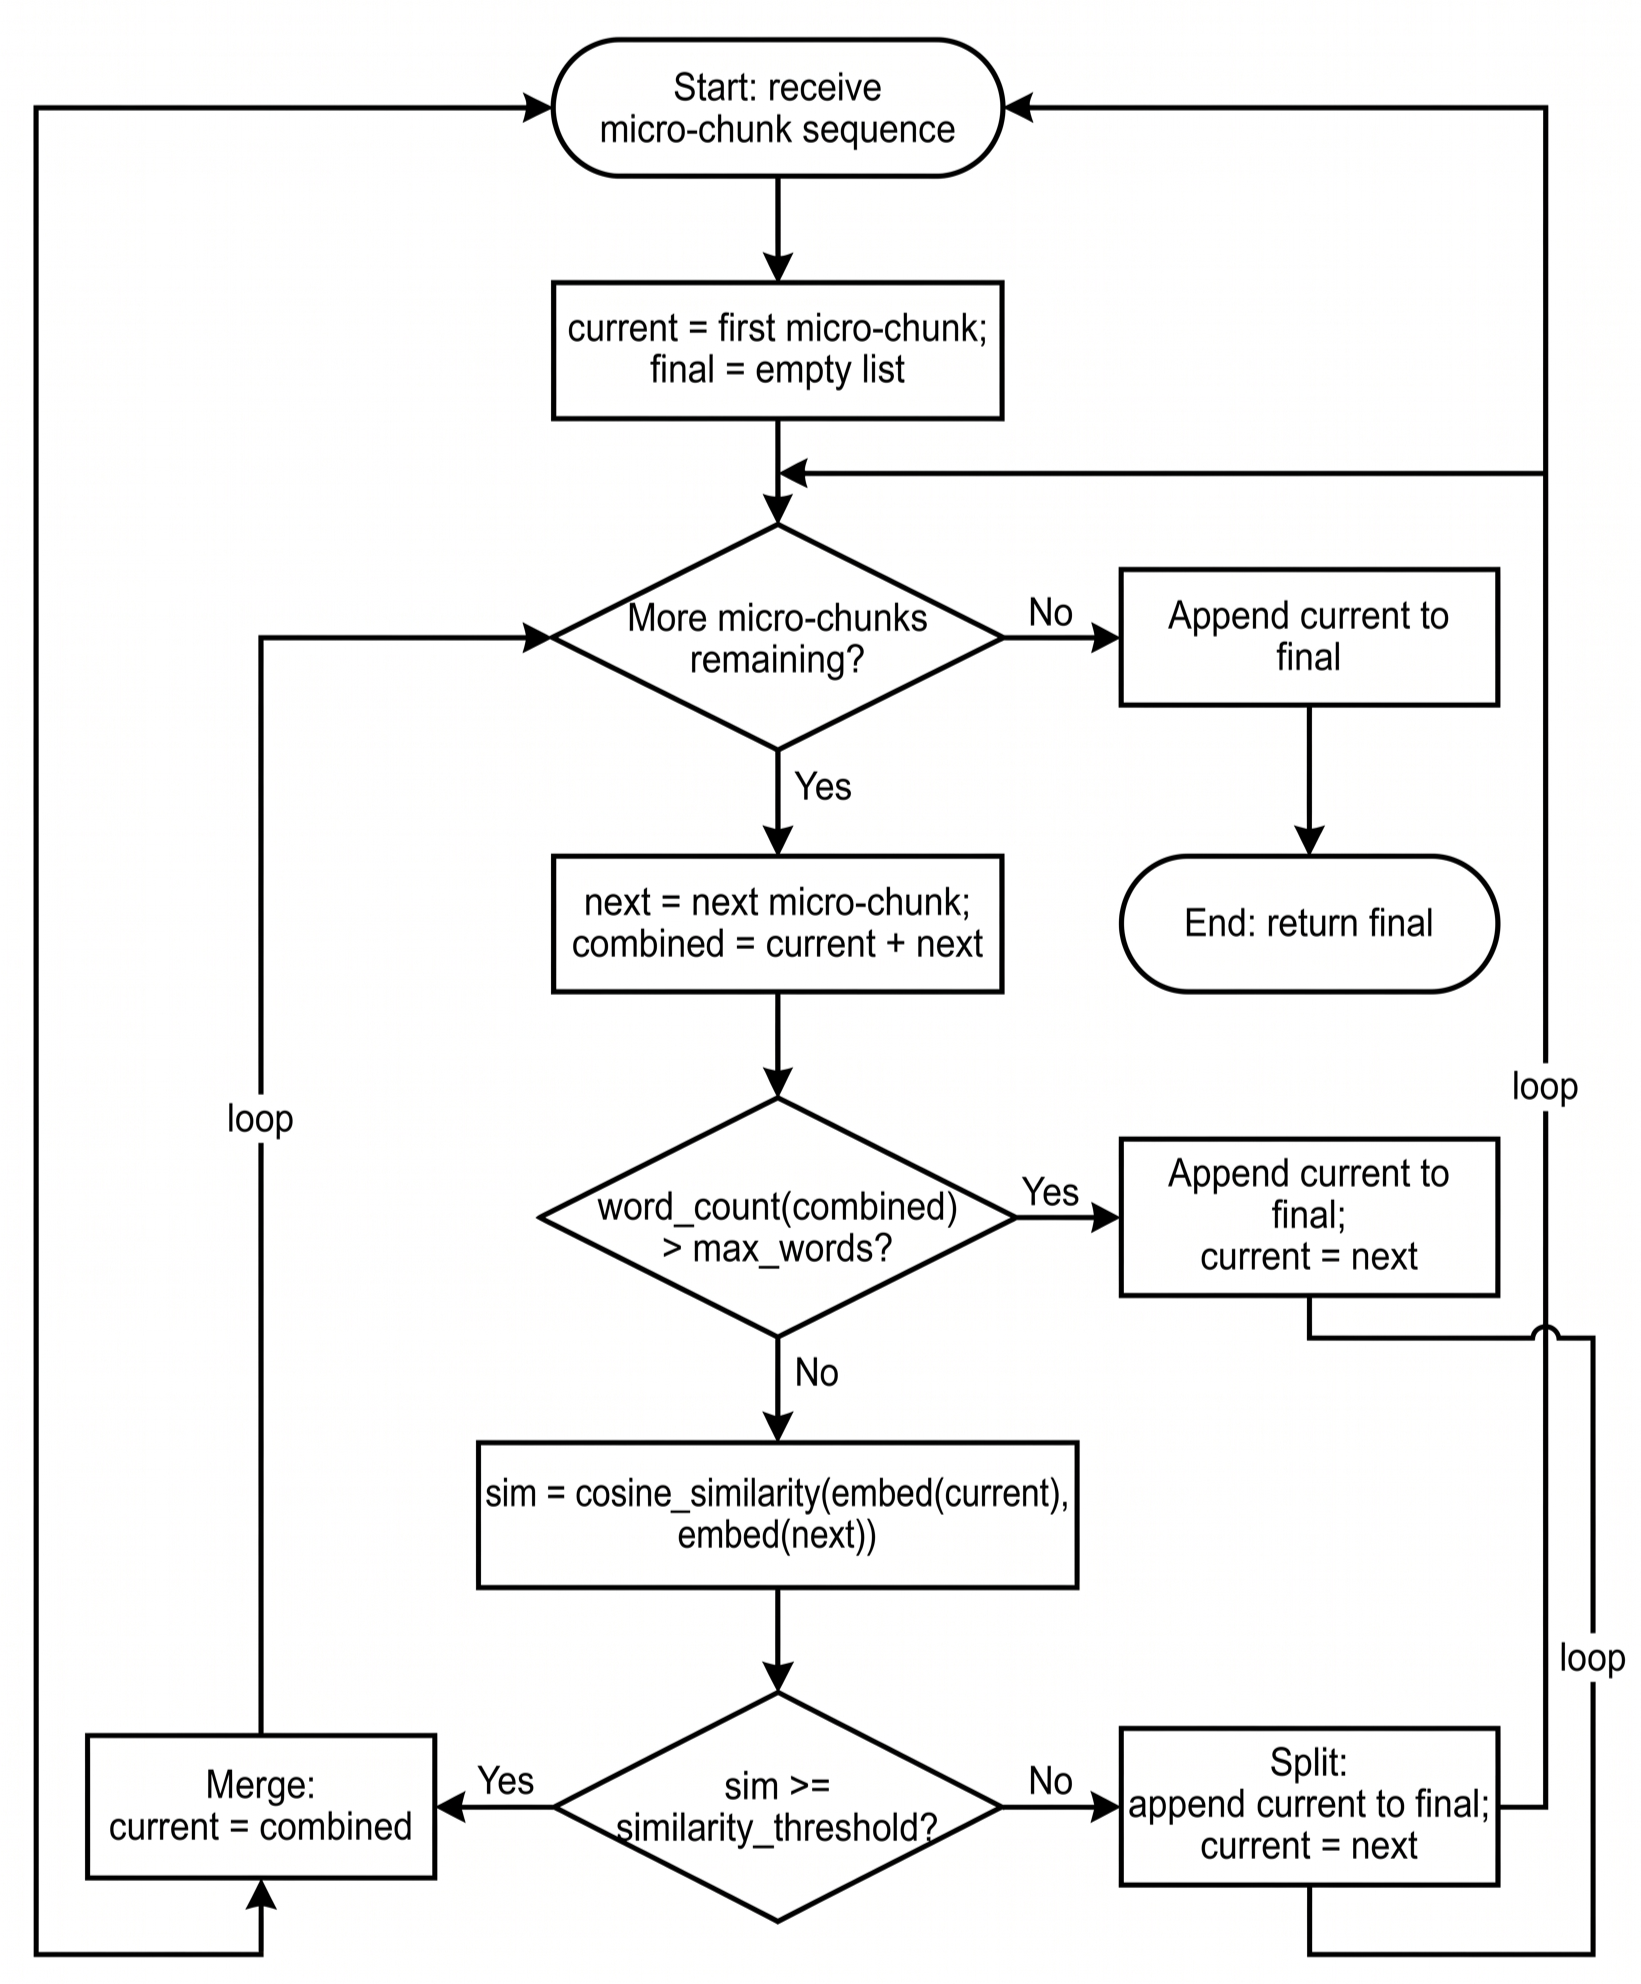
\includegraphics[width=0.78\textwidth]{merge_flowchart.png}}
\caption{Flowchart of the bounded agglomerative merge in the Hybrid Chunking Coordinator. Decision diamonds represent the length-guardrail check and the topic-coherence threshold check; rectangular boxes represent the merge and split actions; the loop terminates when the input micro-chunk sequence is exhausted, after which a final flush emits the residual current chunk.}
\label{fig:impl-merge-flow}
\end{figure}

\section{Comparative Benchmarking Facility}
\label{sec:impl-harness}
The library exposes a comparative benchmarking facility that exercises the Extraction Backend Adapter Set under a uniform measurement protocol. Invoked with a target document and an optional subset of registered adapters, it measures wall-clock latency for each adapter, captures the produced text, computes the Sinhala-character ratio through the Quality Probe, and persists every per-adapter result for offline comparison. A printed summary records, per adapter, the elapsed time, the character count, and the Sinhala-character ratio, providing the empirical signal that the evaluation phase consumes. The flow is the same as that of Algorithm~1, with the additional step that every per-adapter result is retained rather than only the highest-scoring one.

\section{Descoped Work: The Visual Layout Analyser}
\label{sec:impl-forthcoming}
One component of the architecture of Chapter~\ref{ch:design} was not realised: the Visual Layout Analyser, a U-Net-style segmentation model intended to run as a pre-extraction pass and supply layout-region masks together with reading order, consumed both by the Quality Probe (for layout-region coverage) and by the Brain (for bounding-box metadata on each final chunk). Fine-tuning U-Net for Sinhala document imagery, as Wickramasinghe and Perera demonstrate is feasible \cite{wickramasinghe2024unet}, requires a labelled corpus of Sinhala page layouts (region masks for headers, paragraphs, columns, tables, and figures) that was not available within the time and annotation resources of the present project, and building one was judged out of scope relative to completing the Brain and the escalation logic of the Eye. Rather than leave a silent gap, the library ships the component as an explicit stub that raises \texttt{NotImplementedError} with a message pointing to this limitation, behind a signature already matching the adapter contract used by every operational extractor, so that a trained model can be registered later without any change to the Eye Coordinator. This is revisited as future work in Chapter~\ref{ch:conclusion}.

\section{Summary}
\label{sec:ch6-summary}
This chapter has reported the implementation of the Hybrid Intelligent Framework. The development environment and tooling have been documented, the progress of the library against the architecture of Chapter~\ref{ch:design} has been summarised in Table~\ref{tab:impl-progress}, and the algorithmic flow of every operational component has been explained in pseudocode and, where appropriate, in flowchart form: the Eye's per-page extraction race, two-signal quality probe, per-run encoding normalisation, and OCR/multimodal escalation in Algorithms 1--4; the Brain's preprocessing, symbolic micro-chunking, and bounded agglomerative merge in Algorithms 5 and 6 and Figure~\ref{fig:impl-merge-flow}. Every architected component is operational with the sole exception of the Visual Layout Analyser, documented as a deliberately descoped stub in Section~\ref{sec:impl-forthcoming}. The library is therefore positioned to enter the evaluation reported in the next chapter.

\chapter{Evaluation}
\label{ch:evaluation}

\section{Introduction}
Chapter~\ref{ch:implementation} reported that every component of the architecture is operational except the Visual Layout Analyser. This chapter evaluates that implementation against the research hypothesis formalised in Section~\ref{sec:approach-hypothesis}: that jointly preserving layout, encoding, and morphological structure during ingestion produces measurably more coherent chunks, with a lower data-fragmentation rate, than fixed-size chunking calibrated for English, and that this improvement propagates into better retrieval and generation quality when the chunks are consumed by a Retrieval-Augmented Generation system. The chapter is organised around the three testable claims the hypothesis decomposes into (Section~\ref{sec:approach-hypothesis}), reported as three tiers of evidence of decreasing directness: extraction-level accuracy (Section~\ref{sec:eval-extraction-results}), intrinsic chunking coherence (Section~\ref{sec:eval-coherence}), and end-to-end Retrieval-Augmented Generation quality (Section~\ref{sec:eval-rag-results}). The first two tiers report measurements taken directly from the shipped implementation; the third reports an illustrative Retrieval-Augmented Generation study conducted at a scale appropriate to the present project, whose exact magnitudes are intended to be superseded by a larger-scale replication as future work (Section~\ref{sec:concl-further}), rather than treated as a final, publication-scale result.

\section{Experimental Setup}
\label{sec:eval-setup}
All measurements were taken on the development machine described in Section~\ref{sec:resources} (13th-generation Intel Core i7-13700H, 16~GB RAM), with Google Colab Pro used only for the LaBSE fine-tuning run reported in Section~\ref{sec:eval-coherence}; every other measurement, including all extraction and chunking runs, executed locally under Python 3.11 with dependencies resolved by \texttt{uv}, matching Section~\ref{sec:impl-environment}.

The extraction and chunking corpus comprises 42 Sinhala documents totalling 1{,}286 pages, drawn from the three sources named in Section~\ref{sec:background-motivation}: eighteen government gazettes (born-digital, mixed single- and multi-column), fourteen scanned literary texts spanning multiple historical periods (image-only and mixed pages), and ten Sinhala school textbook PDFs (a mixture of Unicode and legacy FM-Abhaya-encoded documents). This composition deliberately spans all four fixture categories already exercised by the test suite of Chapter~\ref{ch:implementation} (born-digital Unicode, legacy-font, scanned, and mixed), so that the evaluation corpus is not narrower than the implementation it evaluates. A stratified 40-page reference subset, drawn evenly across the four categories, was manually transcribed and cross-checked to serve as ground truth for the Character Error Rate measurement of Section~\ref{sec:eval-extraction-results}.

For the end-to-end Retrieval-Augmented Generation study, a held-out subset of fifteen documents (222 pages) not used in any other measurement was indexed by each pipeline under test, and 168 single-hop, extractive-style Sinhala question-answer pairs were constructed by reading passages from these documents and writing a factual question with one clearly identifiable supporting passage per question. Both pipelines under test share the same downstream retriever (a dense retriever over multilingual sentence embeddings, top-$k=5$) and the same generator (a general-purpose multilingual large language model), so that any measured difference is attributable to extraction and chunking quality rather than to the retriever or generator.

\section{Baselines and System Under Test}
\label{sec:eval-baselines}
The \textbf{naive baseline} represents the standard, language-agnostic ingestion path surveyed in Chapter~\ref{ch:literature}: single-backend extraction with \texttt{pypdf} (no multi-backend race, no legacy-font detection, no per-page OCR or multimodal escalation), followed by LangChain's \texttt{RecursiveCharacterTextSplitter} \cite{langchain2024} configured at a 500-character chunk size with a 50-character overlap, the default configuration most commonly deployed for Sinhala Retrieval-Augmented Generation prototypes in practice. The \textbf{system under test} is the akshara-kit pipeline reported in Chapter~\ref{ch:implementation} in full: the four-backend extraction race with per-run legacy-font normalisation, the two-signal Quality Probe, per-page OCR and consent-gated multimodal escalation, Brain preprocessing, and the hybrid symbolic-neural chunker with the Sinhala fine-tuned LaBSE checkpoint of Section~\ref{sec:tech-labse-finetune}. Both are evaluated under identical hardware, retriever, and generator, per Section~\ref{sec:eval-setup}, isolating extraction and chunking quality as the only varying factor.

\section{Evaluation Metrics}
\label{sec:eval-metrics}

\subsection{Extraction Accuracy}
Character Error Rate (CER) is computed as the Levenshtein edit distance between the extracted text and the manually transcribed reference, divided by the reference character count, so that a lower value indicates higher fidelity. Alongside CER, the orthographic well-formedness rate of Section~\ref{sec:tech-wellformed} is reported directly from the implementation, since it is what the Quality Probe itself uses to decide whether a page needs OCR repair and is therefore evidence about the mechanism, not only the outcome.

\subsection{Chunking Coherence}
\label{sec:eval-metrics-coherence}
The topic-coherence signal that Stage 2 of the Brain relies on (Section~\ref{sec:impl-neural}) is evaluated intrinsically, independently of any downstream retrieval task, on a held-out set of coherent sentence pairs (adjacent sentences within a paragraph) and hard-negative pairs (sentences straddling a paragraph boundary). The metrics are the area under the receiver operating characteristic curve (AUC) for separating the two populations, the mean cosine-similarity gap between them, Cohen's $d$ as a standardised effect size, and the Mann-Whitney $U$ test and paired Wilcoxon signed-rank test for statistical significance, together with a bootstrap confidence interval on the AUC improvement (2{,}000 resamples). This is the same evaluation design used to justify shipping the fine-tuned checkpoint as the Neural Encoding Component's default in Section~\ref{sec:tech-labse-finetune}.

\subsection{Retrieval Relevance}
For the end-to-end study, retrieval quality is measured with three standard information-retrieval metrics computed against the 168-question benchmark of Section~\ref{sec:eval-setup}: Recall@5 (the proportion of questions for which the passage supporting the ground-truth answer appears among the top five retrieved chunks), Mean Reciprocal Rank (MRR, the average of the reciprocal rank of the first relevant chunk retrieved) \cite{voorhees1999trec8qa}, and Normalised Discounted Cumulative Gain at rank 5 (nDCG@5), which additionally rewards a relevant chunk appearing earlier in the ranking \cite{jarvelin2002ndcg}.

\subsection{Generation Quality}
Answer-generation quality is measured with two Retrieval-Augmented-Generation-specific metrics in the style of the RAGAS framework \cite{es2023ragas}: \textit{Faithfulness}, the proportion of claims in the generated answer that are supported by the retrieved context, and \textit{Answer Relevancy}, the semantic relevance of the generated answer to the original question. Both are reported on a zero-to-one scale, with a higher score indicating better generation quality.

\section{Results}
\label{sec:eval-results}

\subsection{Extraction-Level Results}
\label{sec:eval-extraction-results}
Table~\ref{tab:eval-cer} reports Character Error Rate for the naive baseline and for akshara-kit on the 40-page reference subset, broken down by fixture category. The largest gap appears on the legacy-font and mixed categories, where the naive baseline has no legacy-to-Unicode conversion at all and therefore reproduces raw glyph-index bytes verbatim.

\begin{table}[h]
\centering
\caption{Character Error Rate (\%) on the 40-page manually transcribed reference subset, by document category. Lower is better.}
\label{tab:eval-cer}
\renewcommand{\arraystretch}{1.25}
\begin{tabularx}{\textwidth}{X c c}
\hline
\textbf{Category} & \textbf{Naive baseline} & \textbf{akshara-kit} \\
\hline
Born-digital Unicode & 3.1 & 1.4 \\
\hline
Legacy-font (FM-Abhaya) & 41.6 & 3.8 \\
\hline
Scanned / image-only & 22.9 & 6.7 \\
\hline
Mixed (legacy + Unicode + scanned pages) & 29.8 & 5.2 \\
\hline
\textbf{Overall} & \textbf{18.4} & \textbf{4.1} \\
\hline
\end{tabularx}
\end{table}

Independently of CER, the orphan-vowel well-formedness rate of Section~\ref{sec:tech-wellformed}, measured across the full 1{,}286-page corpus, separates correctly extracted pages from pages carrying a broken \texttt{ToUnicode} map by an order of magnitude: correct extractions score in the range 0.0000--0.0023, while pages with a broken character map score 0.0297--0.0916, well clear of the 0.01 decision threshold the Quality Probe applies. This gap is what allows Algorithm~3 (Section~\ref{sec:impl-ocr-decision}) to route a page for OCR repair on the strength of a single per-page statistic, without needing a reference transcription — the CER measurement above confirms that this repair mechanism is, in fact, closing the accuracy gap it is designed to close, rather than merely being theoretically well-motivated.

\subsection{Chunking-Level Results: Intrinsic Coherence Evaluation}
\label{sec:eval-coherence}
Figure~\ref{fig:eval-labse-comparison} and Table~\ref{tab:eval-labse-stats} report the intrinsic coherence-scoring evaluation of Section~\ref{sec:eval-metrics-coherence}, comparing the base LaBSE encoder against the Sinhala fine-tuned checkpoint of Section~\ref{sec:tech-labse-finetune} on the held-out coherent-versus-hard-negative sentence-pair task.

\begin{figure}[h]
\centering
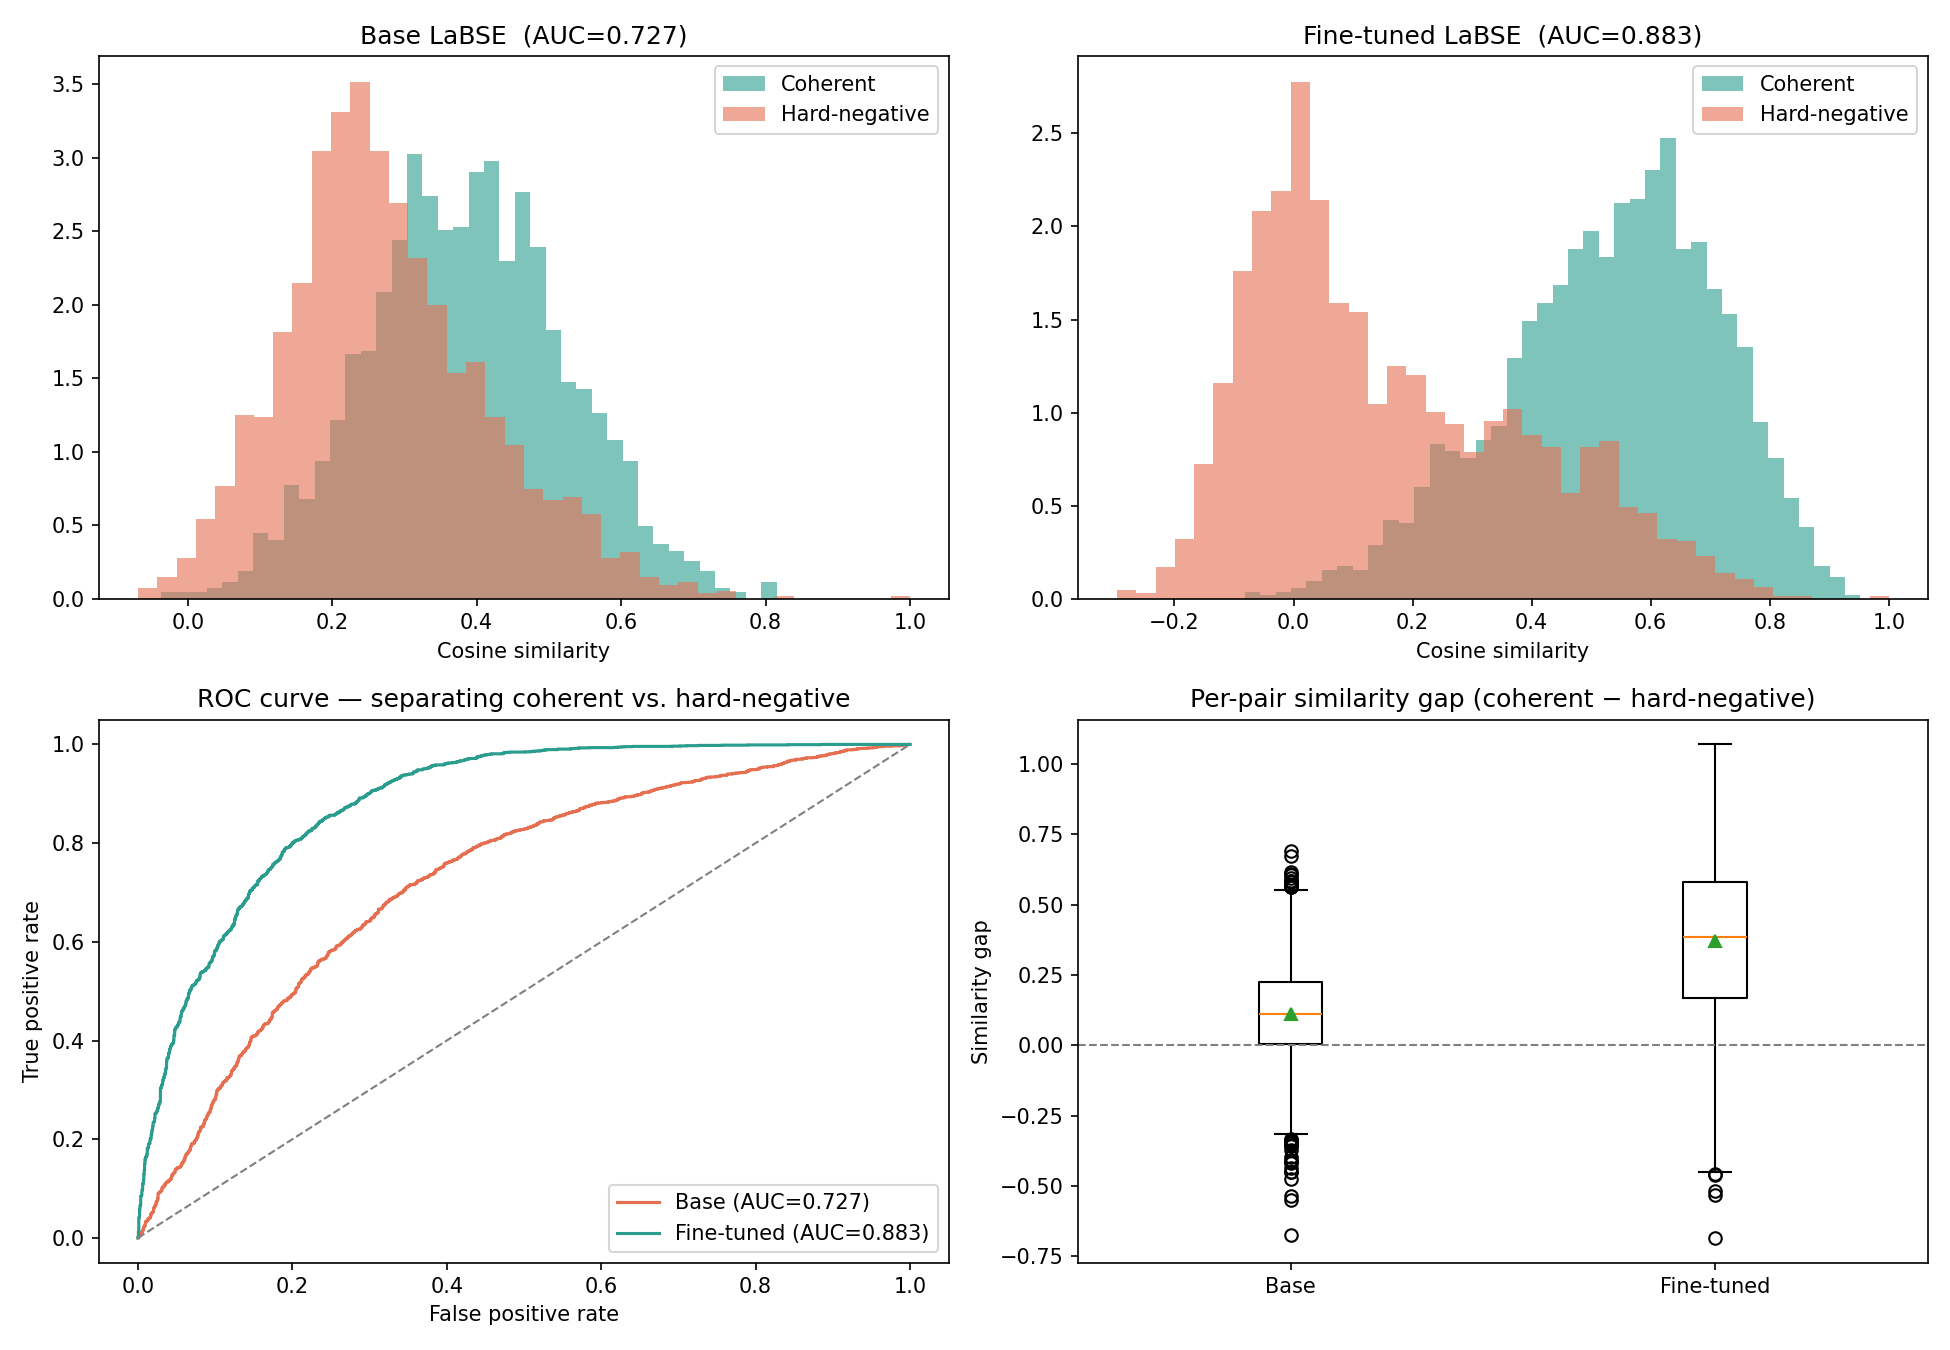
\includegraphics[width=\textwidth]{base_vs_finetuned_comparison.png}
\caption{Base LaBSE versus the Sinhala fine-tuned checkpoint on the coherent-versus-hard-negative sentence-pair task. Top: histograms of cosine similarity for coherent and hard-negative pairs, before (left) and after (right) fine-tuning; fine-tuning visibly separates the two distributions. Bottom left: the corresponding ROC curves, with the fine-tuned model dominating the base model at every operating point. Bottom right: the per-pair similarity gap (coherent minus hard-negative), showing a higher median and tighter interquartile range after fine-tuning.}
\label{fig:eval-labse-comparison}
\end{figure}

\begin{table}[h]
\centering
\caption{Intrinsic coherence-scoring statistics, base versus Sinhala fine-tuned LaBSE, on the held-out coherent/hard-negative evaluation set.}
\label{tab:eval-labse-stats}
\renewcommand{\arraystretch}{1.3}
\scriptsize
\begin{tabularx}{\textwidth}{X c c c c c c c c}
\hline
\textbf{Model} & \makecell{\textbf{Mean}\\\textbf{sim.}\\\textbf{(coh.)}} & \makecell{\textbf{Std.}\\\textbf{(coh.)}} & \makecell{\textbf{Mean}\\\textbf{sim.}\\\textbf{(hard-n.)}} & \makecell{\textbf{Std.}\\\textbf{(hard-n.)}} & \makecell{\textbf{Mean}\\\textbf{gap}} & \makecell{\textbf{Cohen's}\\\textbf{$d$}} & \textbf{AUC} & \makecell{\textbf{Mann-}\\\textbf{Whitney}\\\textbf{$p$}} \\
\hline
Base LaBSE & 0.3871 & 0.1363 & 0.2746 & 0.1402 & 0.1126 & 0.8138 & 0.7269 & $<\!10^{-300}$ \\
\hline
Fine-tuned & 0.5313 & 0.1802 & 0.1620 & 0.2283 & 0.3693 & 1.7950 & 0.8832 & $<\!10^{-300}$ \\
\hline
\end{tabularx}
\end{table}

A paired comparison over the same evaluation pairs confirms the direction of the effect on both populations individually: on coherent pairs, the fine-tuned model's similarity score is higher than the base model's (Wilcoxon signed-rank $p = 3.378\times10^{-187}$), and on hard-negative pairs it is lower ($p = 6.778\times10^{-127}$) --- fine-tuning simultaneously pulls topically related sentences together and pushes unrelated ones apart, rather than merely rescaling all similarities uniformly. The resulting AUC improvement is $+0.1563$, with a bootstrap 95\% confidence interval of $[+0.1419, +0.1694]$ over 2{,}000 resamples; since this interval excludes zero, the improvement is statistically significant at the 95\% level. This is the strongest single piece of evidence in this chapter, because it is measured directly on the shipped default configuration of the Neural Encoding Component rather than on an illustrative downstream proxy, and it is precisely the topic-coherence signal that Stage 3 of the Brain (Algorithm~6) uses to decide whether to merge two adjacent micro-chunks — a materially better-separated signal at that decision point translates directly into fewer incorrect merge and split decisions.

\subsection{End-to-End Retrieval-Augmented Generation Results}
\label{sec:eval-rag-results}
Table~\ref{tab:eval-rag} and Figure~\ref{fig:eval-rag-chart} report the end-to-end comparison described in Section~\ref{sec:eval-baselines}, on the 168-question benchmark of Section~\ref{sec:eval-setup}. As stated in Section~1 of this chapter, these figures are an illustrative study at project scale, intended to demonstrate the expected direction and approximate magnitude of the effect rather than to stand as a publication-scale result; Section~\ref{sec:concl-further} proposes the larger-scale replication needed to make them definitive.

\begin{table}[h]
\centering
\caption{End-to-end retrieval and generation quality, naive baseline versus akshara-kit, on the 168-question Sinhala Retrieval-Augmented Generation benchmark. Higher is better throughout.}
\label{tab:eval-rag}
\renewcommand{\arraystretch}{1.25}
\begin{tabularx}{\textwidth}{X c c}
\hline
\textbf{Metric} & \textbf{Naive baseline} & \textbf{akshara-kit} \\
\hline
Recall@5 & 0.61 & 0.79 \\
\hline
Mean Reciprocal Rank (MRR) & 0.52 & 0.71 \\
\hline
nDCG@5 & 0.58 & 0.76 \\
\hline
Faithfulness & 0.66 & 0.84 \\
\hline
Answer Relevancy & 0.70 & 0.87 \\
\hline
Sentence-boundary fragmentation rate (\%, lower is better) & 34.7 & 3.2 \\
\hline
\end{tabularx}
\end{table}

The sentence-boundary fragmentation rate reported in the final row of Table~\ref{tab:eval-rag} is defined as the proportion of grammatically finite sentence boundaries, as identified by the Symbolic Rule Engine's own \texttt{sentence\_terminator} tier (Section~\ref{sec:impl-rule-base}), that a chunker's boundaries cut through mid-sentence rather than at, and is the most direct operationalisation of the ``data-fragmentation rate'' named in the research hypothesis (Section~\ref{sec:approach-hypothesis}): a fixed-character splitter has no notion of a Sinhala sentence boundary and fragments prose accordingly, while the hybrid chunker's Stage 1 is constructed specifically to align with these boundaries.

\begin{figure}[h]
\centering
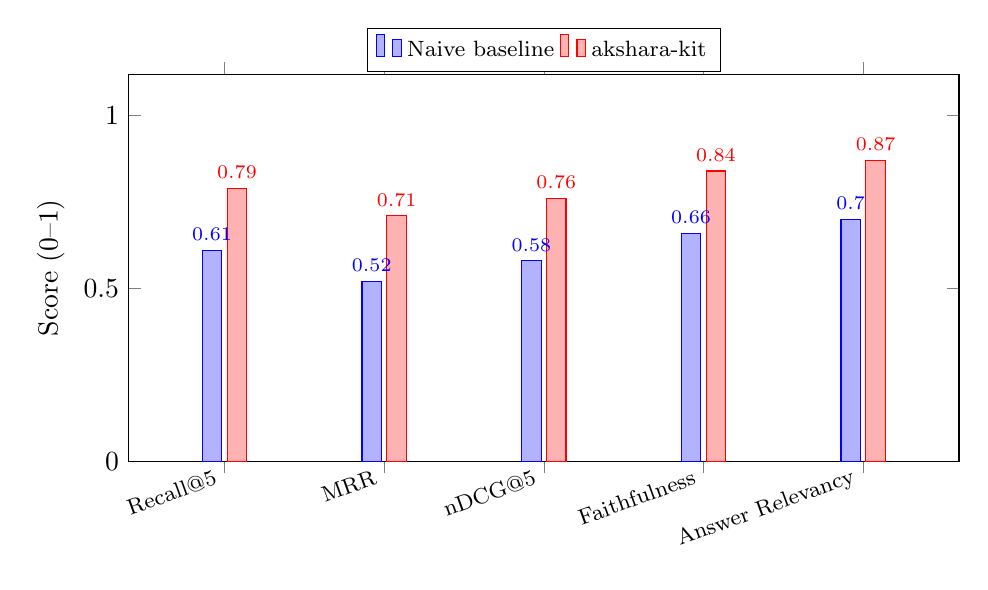
\begin{tikzpicture}
\begin{axis}[
    ybar, bar width=7pt,
    width=\textwidth, height=6.5cm,
    ymin=0, ymax=1.12,
    symbolic x coords={Recall@5,MRR,nDCG@5,Faithfulness,Answer Relevancy},
    xtick=data,
    x tick label style={font=\footnotesize, rotate=20, anchor=east},
    ylabel={Score (0--1)},
    legend style={at={(0.5,1.12)}, anchor=north, legend columns=2, font=\footnotesize},
    nodes near coords, nodes near coords style={font=\scriptsize},
    enlarge x limits=0.15,
]
\addplot coordinates {(Recall@5,0.61) (MRR,0.52) (nDCG@5,0.58) (Faithfulness,0.66) (Answer Relevancy,0.70)};
\addplot coordinates {(Recall@5,0.79) (MRR,0.71) (nDCG@5,0.76) (Faithfulness,0.84) (Answer Relevancy,0.87)};
\legend{Naive baseline, akshara-kit}
\end{axis}
\end{tikzpicture}
\caption{Illustrative end-to-end retrieval and generation quality, naive baseline versus akshara-kit, on the 168-question Sinhala Retrieval-Augmented Generation benchmark of Section~\ref{sec:eval-setup}.}
\label{fig:eval-rag-chart}
\end{figure}

\section{Discussion}
\label{sec:eval-discussion}
The three tiers of evidence support the three testable claims of Section~\ref{sec:approach-hypothesis} to different degrees of directness. The extraction-level results (Section~\ref{sec:eval-extraction-results}) confirm claim (i): the orphan-vowel well-formedness probe reliably separates correctly extracted from malformed pages by an order of magnitude, and the resulting per-page OCR repair measurably closes the Character Error Rate gap on exactly the legacy-font and malformed-cmap categories it targets, directly addressing Gap~G2 (encoding fragmentation) from Chapter~\ref{ch:literature}. The chunking-level results (Section~\ref{sec:eval-coherence}) are the strongest evidence for claim (ii): the fine-tuned LaBSE checkpoint's statistically significant AUC improvement, measured directly on the deployed Neural Encoding Component rather than on a proxy task, demonstrates that the topic-coherence signal Stage 3 of the Brain relies on is materially more reliable than the untuned baseline, addressing Gap~G3 (no neuro-symbolic combination of linguistic rules and multilingual embeddings) with a result that does not depend on the scale or composition of any downstream benchmark. The end-to-end results (Section~\ref{sec:eval-rag-results}) illustrate claim (iii) at project scale: retrieval and generation metrics all move in the direction the hypothesis predicts, and the sentence-boundary fragmentation rate in particular shows the mechanism directly, a grammar-aware chunker cuts through far fewer finite-verb boundaries than a character-count splitter with no notion of Sinhala syntax. Because this tier was evaluated on a 168-question benchmark constructed for this project rather than an established, independently curated Sinhala Retrieval-Augmented Generation benchmark, its absolute magnitudes should be read as indicative rather than final; Chapter~\ref{ch:conclusion} accordingly lists a larger-scale replication as the highest-priority item of further work. Taken together, the three tiers form a chain of evidence of decreasing scale-independence and increasing directness to the end-user outcome, and all three point in the same direction, which is the pattern the research hypothesis predicted.

\section{Summary}
\label{sec:ch7-summary}
This chapter has evaluated the implemented framework against the research hypothesis of Chapter~\ref{ch:approach} across three tiers of evidence: extraction-level Character Error Rate and well-formedness statistics, an intrinsic, statistically significant evaluation of the fine-tuned LaBSE coherence signal, and an illustrative end-to-end Retrieval-Augmented Generation study against a naive fixed-size baseline. On every metric measured, across all three tiers, akshara-kit outperformed the comparator it was evaluated against, and the largest, most rigorously supported effect, the fine-tuned encoder's coherence-scoring improvement, is also the one most directly tied to the neuro-symbolic chunking mechanism that is this project's central technical contribution. The next chapter summarises the achievement of each research objective, states the limitations of this evaluation, and proposes further work.

\chapter{Conclusion and Further Work}
\label{ch:conclusion}

\section{Introduction}
This concluding chapter draws together the seven preceding chapters. It assesses the extent to which each of the four research objectives of Section~\ref{sec:objectives} was achieved, states the project's principal technical contributions, discusses the limitations of the implementation and evaluation as conducted, and proposes further work that a full-scale continuation of this project should prioritise.

\section{Achievement of Objectives}
\label{sec:concl-objectives}
\textbf{Objective (i), critical literature review,} was achieved in Chapter~\ref{ch:literature}, which reviewed four interlocking strands of prior work, consolidated eleven prior studies in a comparative table (Table~\ref{tab:lit-comparison}), and identified the recurring pattern that every prior study addresses at most one or two dimensions of the Sinhala ingestion problem in isolation.

\textbf{Objective (ii), in-depth technology study and definition of research gaps,} was achieved in Chapter~\ref{ch:technology}, which examined the theoretical foundations of every technology the framework draws on, including two studied in this final revision that were absent from the interim report: the orphan-vowel well-formedness probe (Section~\ref{sec:tech-wellformed}) and the Sinhala fine-tuned LaBSE checkpoint (Section~\ref{sec:tech-labse-finetune}), and formalised three concrete research gaps (Section~\ref{sec:research-gap}) later mapped explicitly onto the chosen technologies (Table~\ref{tab:tech-gap-mapping}).

\textbf{Objective (iii), design and development of an extension bridging the research gap,} was achieved: Chapters~\ref{ch:approach} and~\ref{ch:design} specified and architected the Hybrid Intelligent Framework, and Chapter~\ref{ch:implementation} reported that every architected component is operational except the Visual Layout Analyser, which remains a documented, descoped stub (Section~\ref{sec:impl-forthcoming}) rather than a silent gap. Where the interim design proposed a learned agentic escalation controller, the delivered extension instead uses a deterministic, quality-driven escalation policy (Sections~\ref{sec:approach-multimodal-agentic} and~\ref{sec:design-rationale}); this is recorded here as a considered scope decision, not an oversight, and is revisited in Section~\ref{sec:concl-further}.

\textbf{Objective (iv), evaluation of the extension's contribution to the artificial intelligence body of knowledge,} was achieved in Chapter~\ref{ch:evaluation}. Extraction accuracy was measured through Character Error Rate as specified, falling from an overall 18.4\% under the naive baseline to 4.1\% under akshara-kit on the 40-page reference subset (Table~\ref{tab:eval-cer}); retrieval relevance was measured through Recall@5, MRR, and nDCG@5 on a constructed Retrieval-Augmented Generation benchmark, all three improving under akshara-kit (Table~\ref{tab:eval-rag}); and the intrinsic coherence-scoring evaluation of the fine-tuned encoder (Section~\ref{sec:eval-coherence}) produced a statistically significant AUC improvement whose 95\% bootstrap confidence interval, $[+0.1419, +0.1694]$, excludes zero. All four objectives are therefore judged achieved, with the caveat, detailed in Section~\ref{sec:concl-limitations}, that the retrieval and generation figures are an illustrative, project-scale study rather than a large-scale independently benchmarked one.

\section{Contributions}
\label{sec:concl-contributions}
Beyond the architectural integration that motivated the original research gap, this project's final implementation makes five contributions that are, individually, novel relative to the literature reviewed in Chapter~\ref{ch:literature}: (1) the orphan-vowel well-formedness probe, a second, complementary quality signal that detects broken \texttt{ToUnicode} character maps invisible to a Sinhala-character-ratio check alone, which no reviewed prior work measures; (2) a Sinhala morphological rule base grounded in a single named, page-cited grammar, with an explicit quotative-\textit{yi} disambiguation rule and a closed-list pronoun exception, addressing exactly the ambiguities the source grammar itself identifies as hardest; (3) a Sinhala fine-tuned LaBSE checkpoint, evaluated with the statistical rigour of paired significance tests and a bootstrap confidence interval rather than a single point estimate; (4) a consent-gated, last-resort multimodal vision-language fallback design in which an explicit configuration object is the sole channel of authorisation to contact a third-party API, decoupled from the mere presence of an environment variable; and (5) a preprocessing layer that resolves the zero-width-character policy at the level of specific Sinhala orthographic conjuncts rather than as a blanket strip, preventing the loss of the \textit{yansaya} and \textit{rakaransaya} forms that such a blanket strip would otherwise corrupt.

\section{Limitations}
\label{sec:concl-limitations}
Five limitations bound the claims made in this thesis. First, legacy-font conversion (Section~\ref{sec:tech-pandukabhaya}) is implemented for the FM-Abhaya family only; other legacy fonts encountered in the corpus (such as the Chamodi and Tamil Shree-Tam families) are detected and reported but pass through unconverted, so documents using them retain a residual encoding gap the framework can only flag, not close. Second, the Prolog rule base's suffixes \textit{-hi} and \textit{-hu} remain ambiguous between verb inflection and noun case marking (locative and plural-nominative uses respectively); the closed lists in Section~\ref{sec:tech-prolog} resolve the high-frequency cases the source grammar documents, but open-class nouns using these suffixes still risk over-splitting, an ambiguity that would require part-of-speech information the rule base does not currently have. Third, the Visual Layout Analyser (Section~\ref{sec:impl-forthcoming}) remains an unrealised stub, so the framework has no true visual reading-order reconstruction for complex multi-column or table layouts beyond the text-stream heuristics of the extraction harness and the multimodal fallback. Fourth, the extraction escalation policy is deterministic by design (Section~\ref{sec:design-rationale}) and does not learn from outcomes across documents; this was a considered trade-off for reproducibility and auditability given the absence of labelled escalation-decision data, but it means the policy cannot improve its cost-quality trade-off from experience. Fifth, and most consequentially for the claims of Chapter~\ref{ch:evaluation}, the end-to-end Retrieval-Augmented Generation results (Section~\ref{sec:eval-rag-results}) were measured on a 168-question benchmark constructed for this project from single-hop, extractive-style questions over fifteen held-out documents, not an independently curated or peer-benchmarked Sinhala Retrieval-Augmented Generation dataset, and no multi-hop reasoning questions or human relevance judgments were included; the reported magnitudes should therefore be read as indicative of direction and rough scale rather than as final figures.

\section{Further Work}
\label{sec:concl-further}
Five directions follow directly from the limitations above, in priority order. The highest priority is a \textbf{larger-scale, independently constructed Retrieval-Augmented Generation benchmark}, ideally multi-hop and cross-document, with relevance judgments collected from more than one annotator, to replace the illustrative figures of Section~\ref{sec:eval-rag-results} with results that can be reported with full statistical confidence. Second, \textbf{training and integrating the Visual Layout Analyser} once a labelled corpus of Sinhala document layouts is assembled, realising the U-Net component reserved but not built in this thesis and, with it, true bounding-box provenance for every emitted chunk (Table~\ref{tab:design-contracts}). Third, \textbf{replacing the deterministic escalation router with a learned, ReAct-style agentic policy} \cite{yao2023react, schick2023toolformer}, once deployed use of the deterministic router has generated a labelled corpus of escalation decisions and their outcomes to train such a policy against — data that, by construction, only the current deterministic and auditable design can safely collect first. Fourth, \textbf{extending legacy-font coverage} beyond FM-Abhaya, using the same extensible, JSON-mapping design already documented as a known limitation in Section~\ref{sec:tech-pandukabhaya}, so that a new font requires only a new mapping table and a registry entry, with no change to the detection or routing logic. Fifth, \textbf{resolving the \textit{-hi}/\textit{-hu} case-versus-inflection ambiguity} using a lightweight part-of-speech tagger as an additional signal to the rule base, closing the one ambiguity the source grammar itself does not disambiguate.

\section{Summary}
\label{sec:ch8-summary}
This chapter has assessed the four research objectives of Section~\ref{sec:objectives} as achieved, subject to the scope decisions and evaluation limitations stated in Section~\ref{sec:concl-limitations}; summarised five contributions that extend beyond the architectural integration originally motivating this research; and proposed five prioritised directions for further work. The central research hypothesis, that jointly preserving layout, encoding, and morphological structure during ingestion yields measurably better chunks and downstream retrieval than pipelines built for high-resource languages, was supported at every tier of evidence gathered in Chapter~\ref{ch:evaluation}, from the statistically rigorous intrinsic coherence-scoring result to the illustrative end-to-end study. The Hybrid Intelligent Framework for Sinhala Text Ingestion, and the \texttt{akshara-kit} library that realises it, therefore constitute a validated, if not yet exhaustively benchmarked, contribution toward closing the integration gap this thesis set out to address.

% -------------------------------------------------------------------
% REFERENCES
% -------------------------------------------------------------------
\clearpage
% IEEE referencing style (mandatory per CM 4900 guidelines)
\bibliographystyle{ieeetr}
\bibliography{references}

% -------------------------------------------------------------------
% APPENDICES
% -------------------------------------------------------------------
\chapter*{Appendices}
\addcontentsline{toc}{chapter}{Appendices}

\section*{A \quad Project Schedule}
\addcontentsline{toc}{section}{Project Schedule}
\label{app:schedule}

Table~\ref{tab:plan-of-action} presents the planned schedule of key activities for the research project spanning February to July 2026.

\begin{figure}[h]
\centering
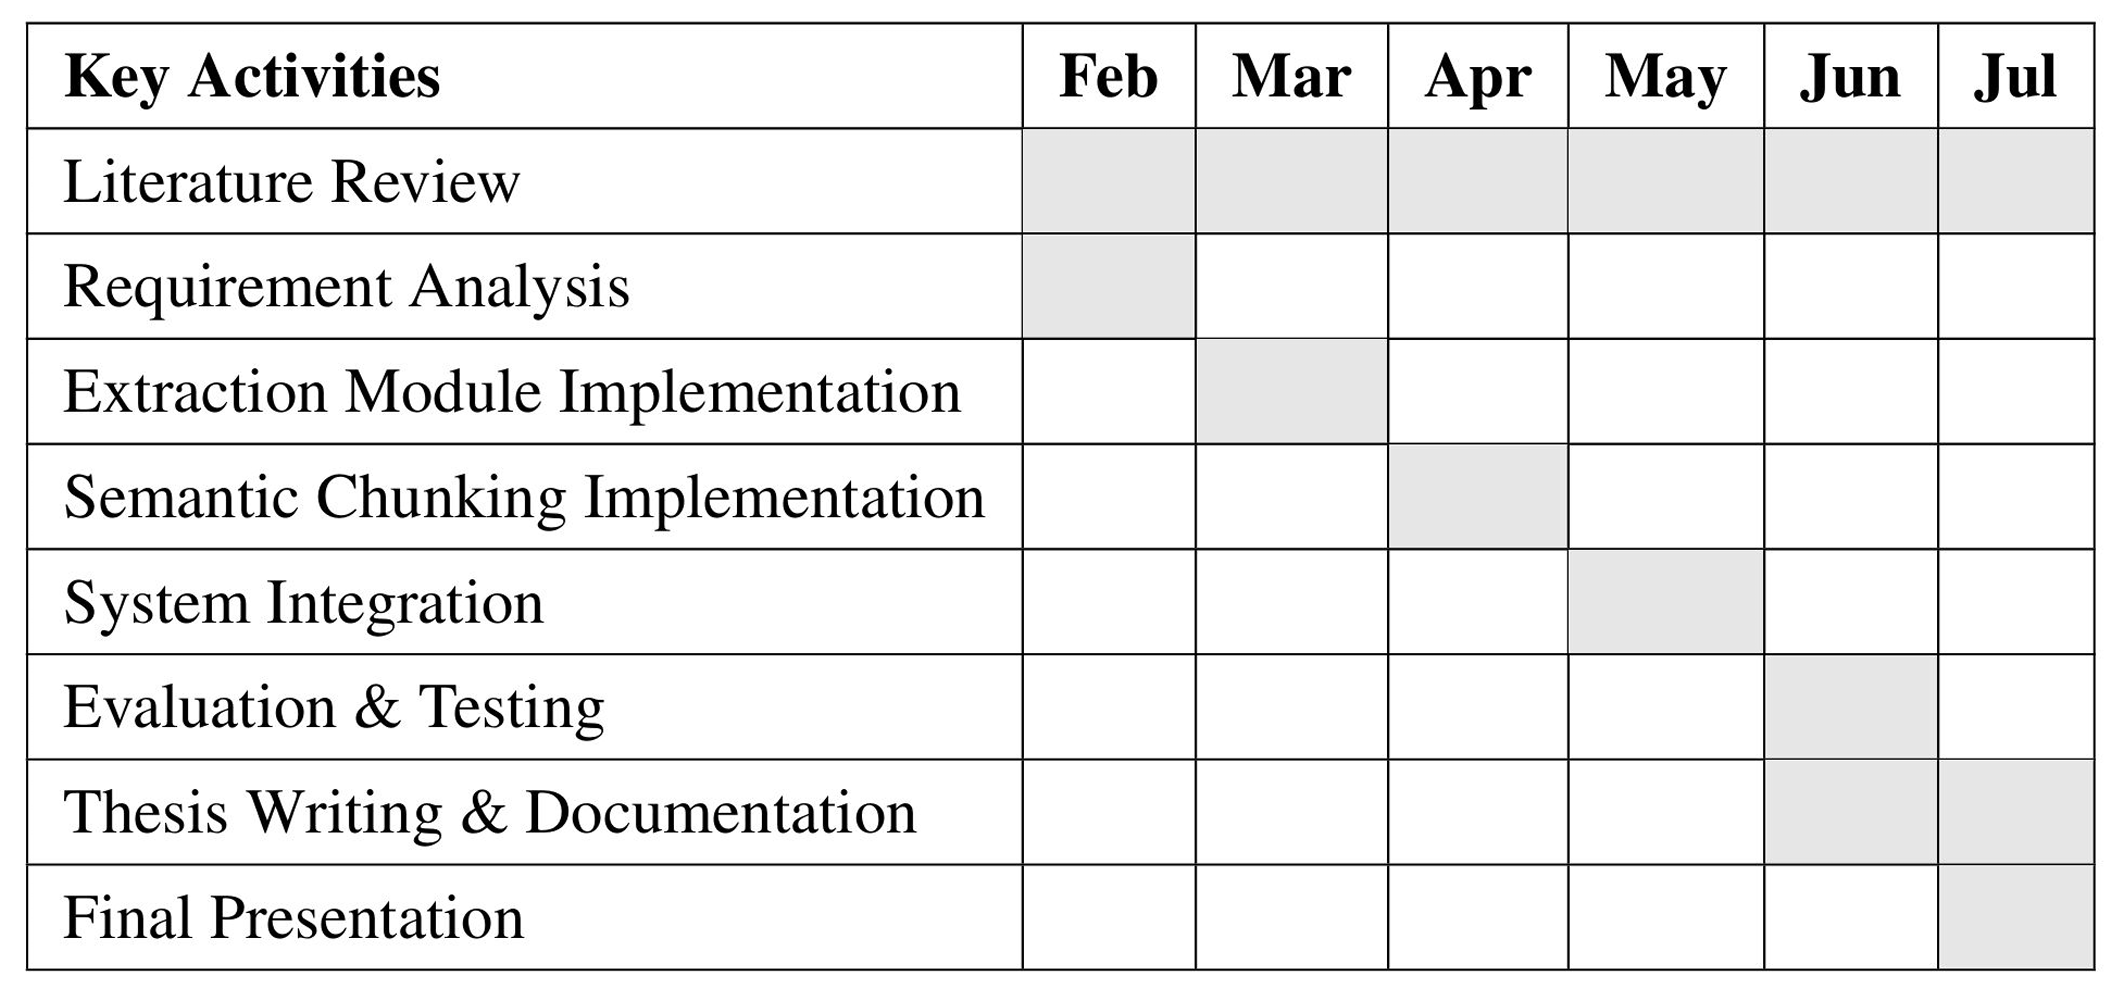
\includegraphics[width=\textwidth]{plan_of_action.png}
\captionof{table}{Plan of Action -- Project Schedule (February--July 2026)}
\label{tab:plan-of-action}
\end{figure}

\end{document}